\section{Motivation and Contribution}

Lobbying and regulatory capture are not merely legislative pressure terms. Organized interests can shape outcomes through campaign finance, public-information distortion, technical comments, litigation delay, procurement design, enforcement priorities, and post-government employment incentives. A useful simulation must therefore model lobbying as an influence economy rather than as a scalar attached to a bill \citep{stigler1971economicRegulation,grossmanHelpman1994,hallDeardorff2006,baumgartner2009lobbying,dalbo2006capture,deFigueiredoRichter2014,bertrand2014whom,carpenterMoss2014}.

This paper contributes an agent-based mechanism model for evaluating anti-capture reforms under strategic channel substitution. When one influence route becomes costly, interests may preserve influence by moving money, expertise, messengers, or pressure into adjacent venues. The model therefore treats reform evaluation as a governance-design problem across disclosure, participation, procedural-integrity, procurement, and enforcement systems. Its main claim is bounded: under transparent substitution assumptions, reform diagnostics can change when evaluation tracks total modeled influence distortion rather than only the observed capture surface. Public administrative data constrain source moments and validation gaps; they are not used here to estimate real-world reform effects. The article follows the tradition of transparent agent-based modeling, where empirical work first constrains ranges and failure modes before supporting policy estimates \citep{epstein1999generative,windrum2007empirical,grimm2010odd}.

\section{Stage-and-Channel Framework}

The model follows a stage-and-channel view of capture. Organized interests can influence electoral selection, legislative agenda setting, agency drafting, notice-and-comment rulemaking, enforcement, litigation, procurement, and implementation. At each stage, the available channels differ: campaign finance is valuable around elections, technical comments and ex parte access are valuable around rulemaking, litigation threats are valuable after an unfavorable rule, and procurement relationships matter during implementation \citep{mccubbins1987administrative,golden1998rulemaking,west2004formal,yackeeYackee2006,gordonHafer2005,kallaBroockman2016,ansolabehere2003littleMoney,baumgartner2009lobbying}.

The central behavioral assumption is channel substitution. When a reform raises the cost of one route, organized interests first try nearby routes that preserve donors, vendors, messengers, relationships, or policy objectives. Direct giving can become outside spending or dark money; registered lobbying can become advisory work; public comments can become sponsored expert submissions or litigation; procurement lobbying can become consulting or subcontracting pressure. The simulator therefore reports both visible channel mix and inferred hidden influence, because some reforms improve one disclosure surface while moving influence elsewhere \citep{dalbo2006capture,carpenterMoss2014,lapiraThomas2017,oecdLobbying2021,brennanDarkMoney2025}.

\section{Theoretical Positioning}

The contribution is not a new general theory of lobbying influence, nor an empirical estimate of capture. It is a computational bridge between three literatures that are usually evaluated separately. Lobbying and capture research identifies channels of access, expertise, money, and institutional vulnerability. Venue-shopping and agenda-setting research shows that organized actors choose institutional settings strategically rather than treating the policy process as one fixed forum \citep{baumgartnerJones1993,pralle2003venue}. Regulatory-governance scholarship emphasizes that modern rule systems are polycentric, with public agencies, private intermediaries, procedural controls, and accountability systems interacting across formal boundaries \citep{black2008polycentric,leviFaur2011regulation}.

Strategic channel substitution matters because anti-capture reforms often target one observable surface at a time. Disclosure, public financing, comment authentication, cooling-off rules, procurement safeguards, and meeting logs can each improve accountability within their own venue, but organized interests may respond by changing messengers, timing, or institutional forum. The model therefore treats reform design as a cross-venue diagnostic problem: a reform should be evaluated not only by the channel it closes, but by whether influence pressure reappears through adjacent money, information, access, procurement, enforcement, or litigation paths. This framing also connects notice-and-comment participation and procedural-control research to the simulator's comment-triage and arena-resolution modules \citep{balla1998administrative,naughton2009commenter}.

The mechanism is useful for regulatory-governance theory because it identifies three recurring design errors. The first is surface substitution: a rule can reduce a measured activity without reducing the underlying capacity to distort public decision making. The second is measurement compression: observed lobbying contacts, campaign contributions, comment counts, procurement awards, and enforcement actions are often reported in separate administrative systems, so a decline in one trace can be mistaken for a decline in total influence pressure. The third is enforcement asymmetry: regulators and watchdogs must detect cross-venue movement, while organized interests need only find one path with enough opacity, credibility, or delay value to preserve the expected return on influence spending. A mechanism model cannot resolve the empirical size of those errors, but it can make their logical consequences explicit.

This also clarifies why the paper uses agent-based simulation rather than a closed-form model. The core question is not whether a single actor spends more when a price changes. It is how a population of organized interests reallocates budgets across channels whose costs, visibility, and institutional returns change at different times. The model's adaptive elements are deliberately modest: lobby organizations learn channel returns, funders increase support when private stakes and reform threats rise, and substitution choices respond to anonymity, messenger credibility, legal cost, setup time, procurement venue value, and cross-venue detection. That is enough to test whether reform diagnostics change when actors can substitute across channels, without requiring a full model of electoral competition or agency preference formation.

\section{Model Overview}

The model contains lobby organizations, public officials, regulators, candidates, enforcement agencies, reform regimes, policy contests, influence arenas, and scenario reports. A policy contest may represent a statute, agency rule, enforcement priority, procurement decision, litigation posture, election pressure point, or anti-capture reform.

The model is agent-based primarily on the influence-supply side: lobby organizations and funders adapt budgets, channel allocations, substitution choices, and defensive spending. Institutional actors are represented through arena susceptibility, reform controls, enforcement probabilities, queue pressure, attention, and backlash parameters.

Each tick follows six steps:

\begin{enumerate}
  \item A policy contest is selected from the scenario's contest mix.
  \item Lobby organizations choose a strategy, evaluate substitution pressure, and allocate finite budgets.
  \item Influence channels modify public support, public benefit, private gain, information distortion, dark-money influence, revolving-door influence, campaign finance influence, litigation threat, comment-record quality, and hidden influence.
  \item The relevant arena resolves the contest under the active reform regime.
  \item Enforcement may detect and sanction capture attempts.
  \item Lobby organizations update strategy memory and issue-specific spending multipliers.
\end{enumerate}

Capture is a synthetic contest-level outcome, not a directly observed legal finding. In the simulator, a non-reform contest is captured when private-gain-weighted pressure, arena susceptibility, information distortion, campaign finance, revolving-door pressure, litigation pressure, hidden substitution, procurement exposure, or comment-record distortion pushes the pre-audit contest score over an arena threshold and enforcement does not reverse it. Anti-capture contests are resolved separately as reform-enactment contests, so the model does not confuse passage of a reform with elimination of capture.

The arena abstraction is intentionally comparative rather than institution-complete. A legislative contest, rulemaking contest, procurement contest, enforcement contest, and litigation contest do not share the same legal procedure, but they can be compared through a small set of common state variables: private gain, public benefit, public salience, susceptibility, information asymmetry, access dependence, enforcement reach, and backlash. Arena-specific code then changes which channels matter most. Technical information and comment authenticity are central in rulemaking. Campaign finance and public financing matter more in electoral pressure contests. Procurement contests give weight to vendor concentration, competition fields, modification exposure, and firewall strength. Enforcement contests give weight to audit probability, sanction severity, and forbearance. Litigation contests give weight to delay value and legal threat.

This abstraction makes the model less detailed than an institutional case study, but it is the reason cross-venue substitution can be evaluated in one system. A direct lobbying ban should not be tested only in a legislative venue if the expected response is to shift toward sponsored technical comments, association intermediaries, procurement consulting, or litigation threats. Likewise, public financing should not be tested only as an electoral subsidy if it changes the marginal value of dark money, intermediary spending, or defensive anti-reform campaigns. The arena layer therefore acts as a translation surface: channel spending is resolved through the institutional features that make that venue vulnerable.

The officials, regulators, candidates, and enforcement agencies in the model are not rich psychological agents. They are institutional targets with heterogeneous susceptibility and procedural controls. This is a limitation, but it is also a scope choice. The article asks how influence-supply actors adapt when reform regimes change. A later version could endogenize public-official learning, agency mission drift, electoral incentives, or prosecutor strategy, but those additions would not remove the need to track cross-channel movement on the influence-supply side.

% Generated by scripts/generate-interaction-figures.py; source=src/main/java/lobbycapture; graphic=Figure_1_model_architecture.pdf
\begin{figure}[tbp]
\centering
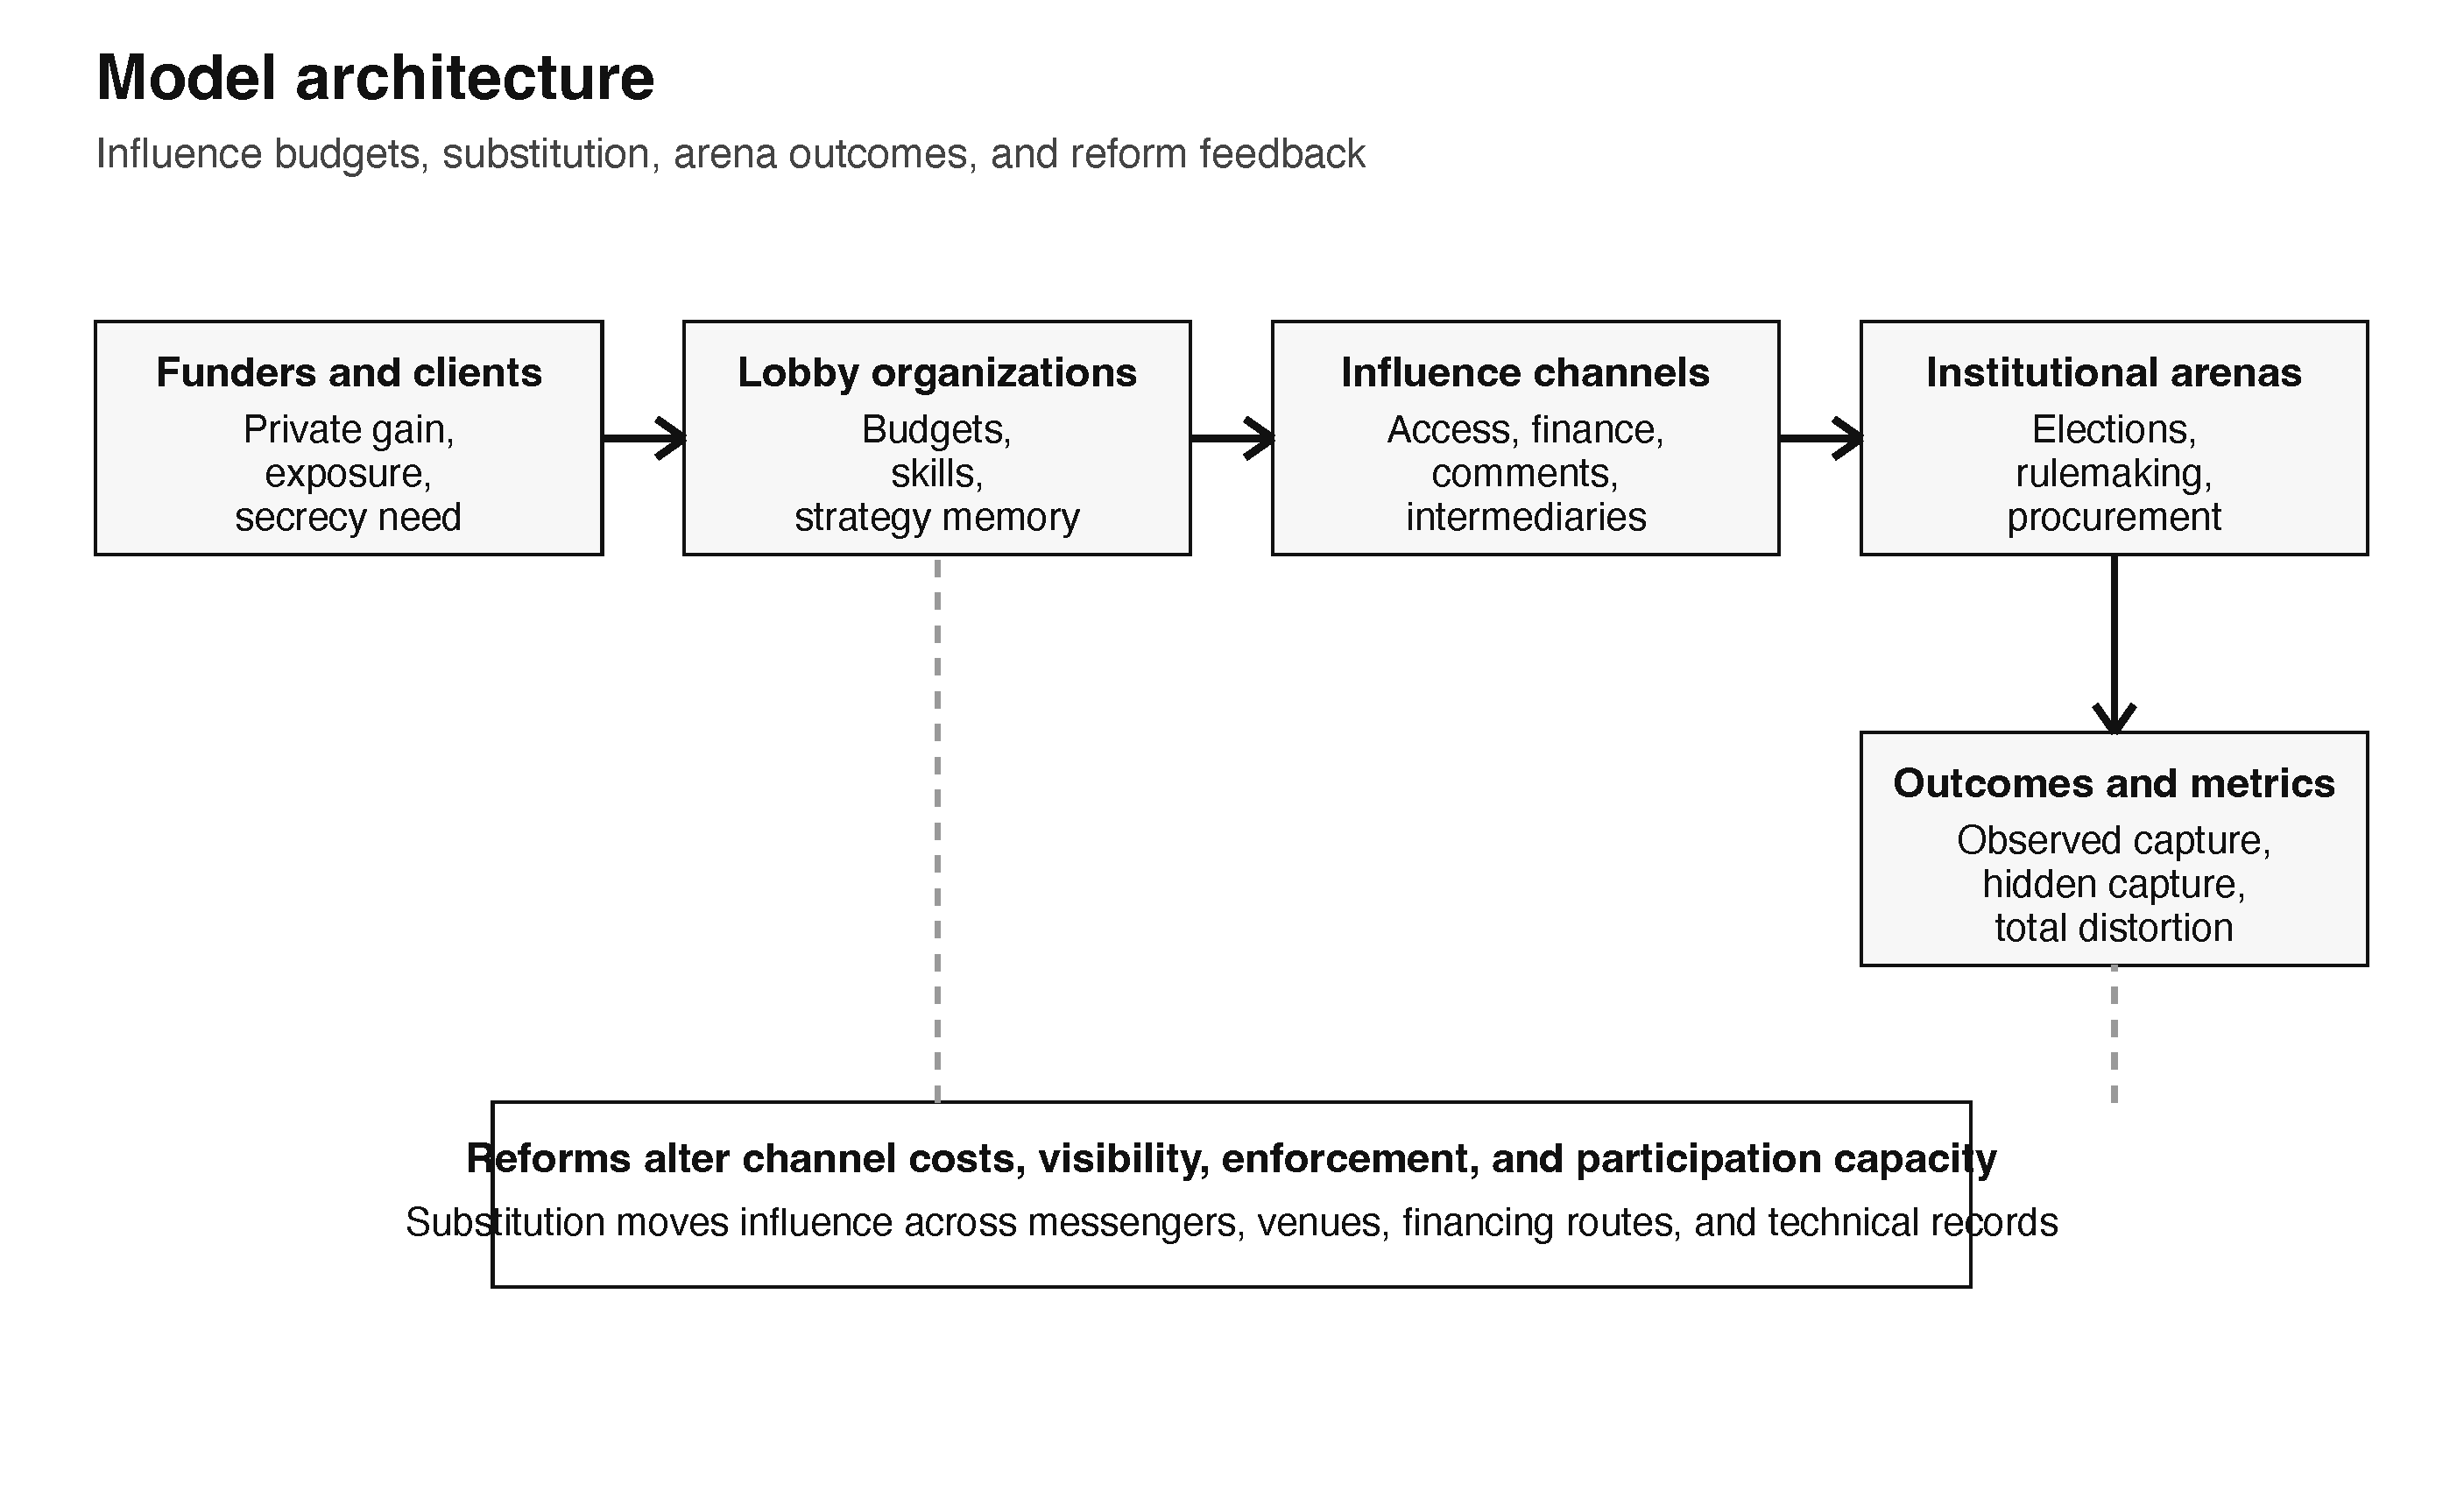
\includegraphics[width=0.95\linewidth]{figures/Figure_1_model_architecture.pdf}
\caption{Model architecture. Funders replenish lobby budgets, lobby organizations allocate spending across visible and hidden channels, arenas resolve contests, and outcome metrics plus enforcement feed back into later strategy.}
\label{fig:model-architecture}
\end{figure}


\begin{table*}[tbp]
\centering
\scriptsize
\setlength{\tabcolsep}{3pt}
\begin{tabular}{p{0.18\textwidth}p{0.30\textwidth}p{0.12\textwidth}p{0.20\textwidth}p{0.13\textwidth}}
\toprule
Quantity & Meaning & Range & Source or rationale & Used in \\
\midrule
Observed capture & Share of resolved non-reform contests crossing the arena capture threshold after enforcement. & 0--1 & Synthetic contest resolution; not an empirical rate. & Outcome diagnostic \\
Hidden influence & Influence preserved through opaque finance, intermediaries, venue shifting, messenger substitution, or defensive adaptation. & 0--1 & Strategy memory, evasion profile, channel mix, and reform leakage. & Substitution diagnostic \\
Hidden capture & Index combining hidden influence, preserved influence, substitution, defensive spending, private gain, policy distortion, procurement bias, and enforcement forbearance. & 0--1 & Mechanism diagnostic; no direct public-data analogue. & Capture audit \\
Total influence distortion & Composite of observed capture, hidden capture, policy distortion, procurement bias, comment flooding, technical distortion, administrative burden, preserved hidden influence, opacity, intermediary load, procurement exposure, and venue shifting. & 0--1 & Lower-is-better design loss; weights are explicit model choices. & Reform comparison \\
Substitution risk & Probability-like diagnostic that a reform suppresses a visible channel while preserving influence elsewhere. & 0--1 & Substitution engine and channel movement. & Warning audit \\
Reporting-error detection & Narrow diagnostic for lobbying-reporting compliance errors likely to enter enforcement, split from broad modeled capture detection. & 0--1 & Disclosure lag, regulated lobbying surface, transparency, audit, and enforcement capacity. & Validation bridge \\
Campaign sanction incidence & Narrow diagnostic for penalty-bearing campaign-finance or outside-spending cases, split from broad per-contest sanctions. & 0--1 & Campaign money exposure, disclosure reach, audit capacity, and sanction severity. & Validation bridge \\
\(E[I]\) & Expected influence from a substitute route. & 0--1 & Learned return memory and scenario profile. & Switch score \\
\(C_m,A_n,V_o\) & Messenger credibility, anonymity value, and vendor or venue overlap. & 0--1 & Scenario and reform profile. & Switch score \\
\(I_m,E_f,R_v,P_v,X_v\) & Intermediary fit, evasion freedom, visible-route restriction, procurement venue value, and cross-venue detection. & 0--1 & Scenario, arena, evasion, procurement, and reform profile. & Switch score \\
\(L_c,D_c,T_s\) & Legal cost, disclosure cost, and setup time. & 0--1 & Reform controls and channel profile. & Switch score \\
Design loss & Illustrative lower-is-better portfolio objective combining total distortion, hidden capture, substitution risk, administrative cost, opacity, chill, speech risk, detection, and participation protection. & 0--1 & Normative screen for stress testing, not a policy welfare estimate. & Portfolio screen \\
\bottomrule
\end{tabular}
\caption{Core model diagnostics and substitution-score terms. All quantities are normalized model variables unless noted otherwise.}
\label{tab:model-specification}
\end{table*}

Table~\ref{tab:composite-weights} gives the implemented composite weights for total influence distortion and design loss. These are transparent model choices rather than estimated welfare weights. Several components are correlated, so the index should be read as a grouped diagnostic screen, not as a decomposition of independent causal effects. The stress tests evaluate rankings under the chosen diagnostic, while supporting materials report equal-weight, hidden-discounted, and burden-heavy diagnostic variants for comparison.

\begin{table*}[tbp]
\centering
\scriptsize
\setlength{\tabcolsep}{3pt}
\begin{tabular*}{\textwidth}{@{\extracolsep{\fill}}lrlr@{}}
\toprule
Total-distortion component & Weight & Design-loss component & Weight \\
\midrule
Observed capture & 0.16 & Total influence distortion & 0.30 \\
Capture pressure index & 0.16 & Hidden capture & 0.20 \\
Hidden capture & 0.15 & Substitution risk & 0.16 \\
Policy distortion & 0.12 & Administrative burden & 0.10 \\
Hidden influence & 0.09 & Network opacity & 0.09 \\
Preserved influence & 0.08 & Legitimate-advocacy chill & 0.07 \\
Procurement bias & 0.07 & Speech-restriction risk & 0.06 \\
Enforcement forbearance & 0.06 & Cross-venue detection & -0.05 \\
Comment flooding & 0.05 & Participation protection & -0.03 \\
Technical rulemaking distortion & 0.04 & & \\
Network opacity & 0.04 & & \\
Intermediary centrality & 0.03 & & \\
Procurement exposure & 0.03 & & \\
Venue-shift load & 0.03 & & \\
Administrative burden & 0.02 & & \\
\bottomrule
\end{tabular*}
\caption{Composite diagnostic weights. Total influence distortion is a clamped additive index over contest outcomes and channel diagnostics. Design loss is a lower-is-better portfolio screen; negative weights reward detection and participation protection.}
\label{tab:composite-weights}
\end{table*}


The composite design is deliberately conservative about interpretation. Total influence distortion is not a social-welfare measure and should not be read as if each component were independently observed. Some components are related by construction: hidden influence contributes to hidden capture; preserved influence can increase venue-shift load; administrative burden can affect public participation and therefore indirectly affect capture risk. The model keeps these terms visible because they represent different governance concerns even when they covary. A reform that reduces observed capture by making participation costly has a different institutional meaning than a reform that reduces observed capture by improving detection, even if both lower a single binary outcome. The composite index therefore functions as a dashboard summary whose components remain auditable in the report tables.

Two safeguards reduce the risk that the model simply rewards its own preferred reform bundle. First, the mechanism comparison disables substitution and compares model modes under the same reform families. Second, the supporting diagnostic-variant tables change switch-score and composite-weight assumptions. These checks do not prove an empirical ranking, but they show whether the qualitative warning depends entirely on one hidden-influence weight or one substitution formula. If a result appears only under the main composite and disappears under hidden-discounted or burden-heavy variants, it should be treated as a design hypothesis rather than a stable mechanism finding.

\section{Actors and Channels}

Lobby organizations are defined by four groups of attributes: issue preferences and client exposure; budget accounts and funding sources; channel skills such as access, technical expertise, public campaigning, litigation, revolving-door networks, and disclosure avoidance; and adaptive parameters such as reform-threat sensitivity, evasion skill, and defensive multipliers. Influence channels are grouped into access, information, public-mobilization, legal-pressure, campaign-finance, dark-money, revolving-door, intermediary, procurement, and defensive-reform routes.

Reform regimes are likewise grouped by function. Disclosure systems alter visibility and traceability; countervailing-participation systems add public financing, vouchers, public-interest representation, or public advocates; procedural-integrity systems include blind review, comment authentication, meeting logs, and anti-astroturf controls; procurement systems add firewalls and venue-shift detection; enforcement systems set audit rates, budgets, sanctions, appeal delay, false-positive cost, and constitutional challenge risk. Full parameter inventories are maintained in the scenario catalog and supporting information.

\section{Strategic Allocation}

The model treats lobbying as a budget allocation problem under institutional constraints. Clients first replenish lobby organizations when expected private gain, exposure, and secrecy needs justify additional spending. For client \(c\), lobby \(l\), issue domain \(d\), and contest \(t\), funding is stylized as

\[
F_{c,l,t} =
\operatorname{clip}\left(k P_{l,d} E_{c,t} S_d (0.35 + G_{c,d} + R_{l,t}), 0, F_{\max}\right),
\]

where \(P_{l,d}\) is lobby issue preference, \(E_{c,t}\) is regulatory, procurement, enforcement, or campaign exposure, \(S_d\) is the calibration issue scale, \(G_{c,d}\) is client private gain, and \(R_{l,t}\) is reform-threat funding pressure for anti-capture contests. Funding enters the lobby budget and is also recorded as a money flow with source type, disclosure lag, traceability, legal risk, reputational risk, and contest linkage.

Lobby organizations then allocate channel spending from their available accounts. Each channel weight combines the active strategy, issue preference, expected return memory, and evasion incentives:

\[
A_{l,j,t} =
\min \left(B_{l,j,t}, I_l P_{l,d} W_{s,j}(1 + M_{l,j})(1 + Q_{j,t})\right),
\]

where \(B_{l,j,t}\) is spendable channel budget, \(I_l\) is influence intensity, \(W_{s,j}\) is the strategy weight for channel \(j\), \(M_{l,j}\) is learned return memory, and \(Q_{j,t}\) is an evasion or reform-threat adjustment. Channel allocations update public support, agenda access, information distortion, campaign influence, dark-money influence, litigation threat, revolving-door influence, and defensive anti-reform pressure. They also generate an influence-network snapshot: weighted paths from funders and lobby organizations through access, campaign finance, dark money, intermediaries, revolving-door relationships, procurement links, comment mobilization, litigation, or defensive-reform pressure to a target domain. The report records network opacity, donor concentration, intermediary centrality, official-access centrality, procurement exposure, revolving-door bridge strength, comment-network load, venue-shift load, and legibility. These are synthetic path diagnostics, but they make substitution more precise: a reform can lower visible contact while increasing opaque intermediary or venue-shifting paths.

Rulemaking contests carry a docket. Comment campaigns are generated from public-campaign, dark-money, information-distortion, and intermediary spending. Anti-astroturf strength raises authentication and reduces synthetic comments; sponsor expertise and information bias affect technical-claim credibility. Intermediary spending can increase sponsored technical submissions and template saturation even when direct lobbying is restricted. The arena then resolves the contest using the resulting docket authenticity, template saturation, and information distortion.

Comment records are triaged before reporting. A docket is divided into a unique-information core, organized technical content, template saturation, and astroturf or misattributed comments. Duplicate compression, authentication confidence, review burden, procedural acknowledgment, and substantive uptake are calculated separately. This reflects the administrative-law design point that raw comment volume is a noisy salience signal, not a measure of evidentiary quality \citep{acusMassComments2021,nyagFakeComments2021}.

The substitution engine calculates a switch score:

\[
\begin{aligned}
S_{l,t} = \operatorname{clip}\bigl(&0.34E[I] + 0.22A_n + 0.18C_m + 0.12V_o\\
&+ 0.08I_m + 0.10E_f + 0.12R_v + 0.08P_v\\
&- 0.18L_c - 0.08D_c - 0.10X_v - 0.10T_s,\ 0,\ 1\bigr).
\end{aligned}
\]

where \(E[I]\) is expected influence under the substitute route, \(A_n\) is anonymity value, \(C_m\) is messenger credibility, \(V_o\) is vendor and relationship overlap, \(I_m\) is intermediary fit, \(E_f\) is evasion freedom, \(R_v\) is visible-route restriction, \(P_v\) is procurement venue value, \(L_c\) is legal cost, \(D_c\) is disclosure cost, \(X_v\) is cross-venue detection, and \(T_s\) is setup time. The result is not a one-for-one channel replacement. Reports summarize substitution pressure, influence preserved, hidden influence, messenger substitution, venue substitution, and net transparency gain.

The weighted switch score is a transparent baseline rather than an estimated behavioral law. All terms are normalized to \([0,1]\), and substitution activates when the score exceeds the scenario threshold. Report CSVs also include equal-weight, anonymity-heavy, and enforcement-cost-heavy alternative switch scores, which are summarized in the supporting information as switch-rule diagnostics.

Reform success is evaluated with a warning-aware diagnostic. Observed capture is the resolved contest outcome. Hidden capture combines hidden influence, preserved influence, messenger and venue substitution, defensive spending, private gain, policy distortion, procurement bias, and enforcement forbearance. Total influence distortion combines observed capture, hidden capture, policy distortion, procurement bias, comment flooding, technical rulemaking distortion, administrative burden, preserved hidden influence, network opacity, intermediary centrality, procurement exposure, and venue-shift load. A reform that lowers observed capture while increasing total distortion is treated as a distortion failure. A reform that lowers observed capture while increasing hidden influence, hidden capture, or substitution risk is reported as a substitution warning rather than a clean success.

Enforcement applies after contest resolution. Detection probability increases with audit rate, enforcement budget, sanctions, public visibility, and evasion legal risk. When detected, sanctions reduce capture effects and add an evasion penalty. This makes evasion valuable only when opacity gains exceed expected enforcement and disclosure costs.

\section{Resolution, Calibration, and Replication Design}

Each arena resolves contests by combining baseline contest vulnerability with arena-specific susceptibility, channel pressure, hidden substitution pressure, public backlash, reform controls, and stochastic noise. For non-reform contests, the implemented capture-pressure score is

\[
C_t = R_t + A_a + I_t + H_t - K_t(1 - L_t) - B_t + \epsilon_t,
\]

where \(R_t\) is contest-level capture risk, \(A_a\) is arena susceptibility, \(I_t\) is weighted information, campaign-finance, revolving-door, and litigation pressure, \(H_t\) is hidden substitution pressure, \(K_t\) is the active reform-control bundle, \(L_t\) is control leakage from hidden and preserved influence, \(B_t\) is public backlash under transparency, and \(\epsilon_t\) is bounded run noise. Capture is recorded only if the pre-audit score crosses the arena threshold and is not reversed by detection and sanctions. Anti-capture contests are resolved separately by comparing the public case for reform against defensive lobbying, litigation delay, and constitutional challenge risk.

The model is initialized from a fixed scenario catalog, a calibration profile, and deterministic source fixtures or normalized public-data snapshots. Randomness enters through contest sampling, channel-allocation variation, process detection, sanctions, and final contest resolution. Each experiment records run counts, contests per run, runtime provenance, source Git state, and calibration checksum. The committed review build uses a stable runtime-provenance label so Java 21 CI rebuilds and local Java runtimes do not rewrite otherwise identical report snapshots. Report CSVs include Wilson intervals for binomial capture and reform-success outcomes plus multi-seed sample standard deviations for capture, hidden influence, and total influence distortion. The main article tables use run-level standard deviations rather than contest-level Wilson intervals as the primary uncertainty diagnostic; Wilson intervals remain in the CSV supplements. Supporting information provides the ODD description, scenario catalog, validation plan, source-panel inventory, and generated-report documentation.

\begingroup
\begin{center}
\begin{minipage}{\textwidth}
\centering
\footnotesize
\setlength{\tabcolsep}{3pt}
\begin{tabular*}{\textwidth}{@{\extracolsep{\fill}}lrrrl@{}}
\toprule
Experiment & Runs & Contests/run & Seed & Purpose \\
\midrule
Mechanism comparison & 40 & 80 & 542 & Isolate substitution across model modes \\
Campaign snapshot & 40 & 80 & 42 & Compare representative scenarios \\
Sensitivity sweep & 30 & 70 & 142 & Vary enforcement, disclosure, financing, and evasion \\
Ablation sweep & 40 & 80 & 242 & Remove reform-bundle components \\
Interaction sweep & 25 & 60 & 342 & Test combined reform settings \\
Portfolio screen & 35 & 70 & 442 & Compare candidate reform bundles \\
\bottomrule
\end{tabular*}
\par\smallskip
\captionsetup{hypcap=false}
\captionof{table}{Experiment and replication design. Experiments after the campaign snapshot use a high-gain stress-test contest mix designed to expose substitution and enforcement leakage.}
\label{tab:experiment-design}
\end{minipage}
\end{center}
\endgroup


\section{Empirical Bridge}

The empirical bridge constrains model inputs and identifies validation gaps. Public data are used to normalize source moments for lobbying, campaign finance, rulemaking comments, procurement, intermediaries, and revolving-door proxies. The resulting simulations remain mechanism tests rather than causal estimates of reform effects.

Normalized source rows constrain only distributional inputs and warning diagnostics. LDA rows constrain issue funding scale, covered-official visibility, agency contact visibility, the source timing input for the lobbying visibility-lag component, and an LDA-derived covered-position revolving-door panel. The model applies a public-visibility transform to that source timing input so archived LDA row age is not treated as the same object as current public visibility. FEC rows include national party committee receipts plus OpenFEC Schedule E independent expenditures and, when enabled, electioneering and communication-cost rows; they constrain donor concentration, outside-spending exposure, electoral-communication coverage, traceability, and a separate campaign visibility-lag component when the relevant panels are present. The report-level \texttt{averageDisclosureLag} remains an operational money-flow blend rather than the validation target for either source family. Public-financing rows include NYC CFB public-funds payments and Seattle Democracy Voucher aggregates, and dark-money or opaque-capacity bridge rows are handled as separate panels rather than silently mixed into ordinary FEC receipts. Source moments now separate IRS EO BMF opaque-capacity rows from bounded non-proxy nonprofit-routing transfer rows; the committed snapshot includes 80 public ProPublica/IRS Schedule I routing rows from a top-EIN slice, while hidden donor identities remain unobserved. Federal Register and Regulations.gov rows constrain docket size, comment authenticity, template saturation, comment flooding, and technical-claim credibility.

USAspending rows constrain procurement identifiers, competition fields, recipient concentration, and agency concentration. Procurement source moments separate award-level competition rows, a top-award bridge, national-volume and stratified USAspending action panels, the archived USAspending bulk transaction summary, and optional SAM.gov Contract Awards rows. The archived bulk summary supplies the preferred public transaction-history denominator for configured agencies. Modification diagnostics are reported as transaction-row incidence, distinct-award incidence, and amount-weighted incidence, because each denominator answers a different source-bridge question. The procurement benchmark crosswalk remaps the old top-contractor range as a high-concentration agency or award-type slice diagnostic rather than a configured-agency aggregate benchmark, and remaps the old ex-post modification range as a delta or stress-screen concept rather than an absolute transaction-incidence benchmark. The codebase includes an opt-in SAM.gov Contract Awards importer for the same procurement action schema, with synchronous offset page-index strata and asynchronous JSON/CSV extract mode for keyed refreshes; that path is now most useful for coding crosswalks, exclusions, offer counts, protests, and firewall overlays. The EPA award slice remains the environmental calibration panel, while the multi-agency bridge, action panels, bulk summary, and benchmark crosswalk supply denominator-mapped procurement diagnostics without being treated as causal SAM/FPDS modification-capture estimates.

Intermediary rows include local campaign-intermediary records, nonprofit and association capacity proxies, and bounded IRS Form 8872 rows for 527 political organizations. The intermediary bridge audit separates local campaign-intermediary rows, nonprofit-capacity proxies, and IRS 527 rows from representative Form 990 nonprofit-routing evidence; the bounded Schedule I rows are carried in the dark-money bridge and are not treated as a representative intermediary network. Revolving-door rows remain proxy-backed through LDA covered-position reports; the revolving-door bridge audit separates those rows from documented post-employment personnel-movement evidence and reports zero documented movement rows in the committed snapshot.

% Generated by scripts/generate-paper-tables.py; source=reports/source-panel-inventory.csv; config=paper/tables.yml
\begin{table*}[tbp]
\centering
\scriptsize
\setlength{\tabcolsep}{2pt}
\begin{tabular*}{\textwidth}{@{\extracolsep{\fill}}lrrrr@{}}
\toprule
Panel & Moment & Snapshot & Fixture & Status \\
\midrule
Direct dark money & darkMoneySourceShare & 0.0249 & 0.0905 & thin \\
Outside spending & outsideSpendingRows & 650.0000 & 2.0000 & usable \\
Public financing & publicFinancingSourceShare & 0.0830 & 0.4269 & thin \\
Intermediaries & intermediaryRows & 853.0000 & 6.0000 & usable \\
Revolving door & revolvingDoorRows & 284.0000 & 14.0000 & thin \\
Proc. IDs & procurementKnownPiidShare & 1.0000 & 1.0000 & usable \\
Proc. mods & procurementExPostModificationShare & 0.0000 & 0.6000 & thin \\
\bottomrule
\end{tabular*}
\caption{Current source-panel coverage. Snapshot values come from the committed normalized 2024 EPA/ENV panel; fixture values are schema and mechanism scaffolds only. Thin, warning, fixture-only, or missing rows are validation gaps rather than negative empirical findings.}
\label{tab:validation-gaps}
\end{table*}


The main text reports categorical snapshot support so readers do not mistake narrow bridge moments for calibrated empirical estimates; numeric source values remain in the source-panel inventory report. The schema-scaffold column shows where mechanisms are exercised but not yet supported by representative public-data coverage. The validation reports also mark \texttt{source\_gap} rows when the available source denominator does not match the benchmark definition. A fixture-only, thin, warning, missing, or \texttt{source\_gap} status is a validation gap; it should not be interpreted as evidence that the mechanism is unimportant in the real world.

The generated claim-boundary audit maps each source panel to its permitted manuscript claim boundary. Its support-level labels distinguish direct-bounded rows from direct/proxy, proxy, denominator-mapped, conditional-direct, and formally weak evidence, so usable source coverage is not automatically treated as representative empirical support. The supporting claim-source dependency table then applies those labels to claim families; bounded families may support mechanism stress tests while still blocking calibrated policy-effect or representative hidden-channel claims.

% Generated by scripts/audit-claim-dependencies.py; source=reports/claim-source-dependency.csv
\begingroup
\begin{center}
\begin{minipage}{\textwidth}
\centering
\scriptsize
\setlength{\tabcolsep}{3pt}
\begin{tabular}{>{\raggedright\arraybackslash}p{0.16\textwidth}>{\raggedright\arraybackslash}p{0.12\textwidth}>{\raggedright\arraybackslash}p{0.24\textwidth}>{\raggedright\arraybackslash}p{0.20\textwidth}>{\raggedright\arraybackslash}p{0.20\textwidth}}
\toprule
Claim tier & Current posture & Permitted use in this article & Claim not supported & Upgrade evidence \\
\midrule
Internal mechanism diagnostics & cleared & Compare model modes, scenario stress tests, substitution warnings, and design diagnostics under stated assumptions. & Do not read synthetic capture, hidden capture, or total distortion as observed misconduct or welfare loss. & Falsification and parameter discipline require linked substitution episodes, but the mechanism claim does not require policy-effect identification. \\
Observable source moments & 4 cleared; 5 bounded families & Use public rows as distributional anchors, schema checks, source-moment diagnostics, and claim-boundary evidence. & Do not generalize bounded panels into representative hidden-channel magnitudes or national public-financing uptake. & Broaden source panels and keep direct, proxy, denominator-mapped, and program-bounded evidence classes separate. \\
Hidden and substitution mechanisms & bounded & Use bounded routing, intermediary, revolving-door, procurement, and missingness diagnostics to stress-test substitution pathways. & Do not claim empirically validated hidden substitution magnitudes, donor identities, or post-employment movement rates. & Add donor-routing coverage, personnel-movement exports, cross-venue actor links, and procurement overlays. \\
Calibrated policy-effect claims & not cleared & Exclude calibrated reform-effect, representative capture-rate, and definitive portfolio-ranking claims from this article. & Do not describe the simulator as estimating which real-world reforms work. & Clear the causal-calibration target matrix (10 open targets) and rerun claim-source audits before upgrading claim strength. \\
\bottomrule
\end{tabular}
\par\smallskip
\captionsetup{hypcap=false}
\captionof{table}{Claim ladder separating synthetic mechanism diagnostics, bounded source moments, hidden-channel mechanisms, and calibration-blocked claim tiers. The statuses are generated from the claim-source dependency and causal-calibration audits.}
\label{tab:claim-ladder}
\end{minipage}
\end{center}
\endgroup


Table~\ref{tab:claim-ladder} is the manuscript-level decision rule. It separates what the paper demonstrates internally from what the public-data bridge can support and from the calibrated policy-effect claims that remain outside scope.

The committed snapshot is a closed-window reproducibility scaffold for the 2024 EPA/ENV slice, not a representative empirical panel. Report builds default to the committed snapshot directory, \path{data/snapshots/2024-env/normalized/}. Exploratory runs can redirect calibration with \path{LOBBY_CAPTURE_CALIBRATION_DIR}. The validation snapshot adds Schedule E outside spending, OpenFEC electioneering and communication-cost rows, NYC CFB public-financing and intermediary rows, Seattle Democracy Voucher rows, IRS EO BMF nonprofit and association capacity rows, bounded IRS Form 8872 rows for 527 political organizations, IRS EO BMF opaque-capacity proxy rows, bounded ProPublica/IRS Schedule I nonprofit-routing rows, USAspending competition fields, UEI and PIID coverage, a multi-agency USAspending top-award bridge, national-volume and stratified USAspending transaction/action panels, an archived USAspending bulk transaction summary, optional separate SAM.gov Contract Awards rows when configured, and LDA rows that identify covered positions in lobbying reports. The snapshot still lacks observed hidden-donor identities, representative national public-financing panels, SAM/FPDS procurement coding crosswalks, representative all-organization Form 990 nonprofit routing beyond the top-EIN Schedule I slice, complete IRS 527 coverage beyond the bounded alphabetic slice, and representative post-employment personnel-movement exports.

The bridge is strongest for observable disclosure surfaces and weakest for the hidden substitution mechanisms that motivate the model. Its value here is architectural and diagnostic rather than validation of hidden-channel magnitudes.

\section{Mechanism Comparison}

The central mechanism is tested with an explicit model-mode comparison. Table~\ref{tab:mechanism-comparison} runs low, moderate, and strong reform families three ways: a single-channel visible-lobbying baseline, a multi-channel model with substitution disabled, and a multi-channel model with substitution enabled. Within each reform family, the comparison isolates the effect of enabling substitution while holding the contest mix and reform setting constant.

% Generated by scripts/generate-paper-tables.py; source=reports/lobby-capture-mechanism-comparison.csv; config=paper/tables.yml; reportGeneratedAt=2026-05-05T00:00:00Z; seed=542; runs=40; contestsPerRun=80
\begin{table*}[tbp]
\centering
\scriptsize
\setlength{\tabcolsep}{1.5pt}
\begin{tabular*}{\textwidth}{@{\extracolsep{\fill}}lrrrrrr@{}}
\toprule
Family & Model & Cap. & Hidden & H cap. & Dist. & Subst. risk \\
\midrule
Low & Visible scalar & 0.732 & 0.000 & 0.004 & 0.264 & 0.033 \\
Low & Multi/no subst. & 0.789 & 0.000 & 0.004 & 0.288 & 0.051 \\
Low & Multi/subst. & 0.892 & 0.223 & 0.121 & 0.396 & 0.245 \\
Moderate & Visible scalar & 0.102 & 0.000 & 0.004 & 0.111 & 0.013 \\
Moderate & Multi/no subst. & 0.177 & 0.000 & 0.004 & 0.141 & 0.033 \\
Moderate & Multi/subst. & 0.819 & 0.315 & 0.144 & 0.371 & 0.257 \\
Strong & Visible scalar & 0.000 & 0.000 & 0.013 & 0.075 & 0.039 \\
Strong & Multi/no subst. & 0.000 & 0.000 & 0.013 & 0.090 & 0.061 \\
Strong & Multi/subst. & 0.512 & 0.436 & 0.175 & 0.294 & 0.307 \\
\bottomrule
\end{tabular*}
\caption{Model-mode comparison across low-, moderate-, and strong-reform families. The rows separate a visible single-channel baseline, a multi-channel model with substitution disabled, and the substitution-enabled model.}
\label{tab:mechanism-comparison}
\end{table*}


The comparison shows why the model is not merely a larger version of a visible-lobbying scalar. Under the low-reform family, all three model modes produce substantial capture, but the substitution-enabled model reports higher hidden influence, hidden capture, total distortion, and substitution risk. In that setting, substitution is not the only source of capture; it amplifies an already vulnerable environment. Under the moderate-reform family, the visible scalar and no-substitution modes suggest that reform pressure has sharply reduced capture, while the substitution-enabled mode remains highly vulnerable. That is the diagnostic situation reform designers most need to notice: the observed channel can look substantially improved while adjacent channels still carry influence pressure. Under the strong-reform family, visible and no-substitution modes suppress observed capture, but the substitution-enabled mode still records substantial capture and hidden influence. That row is a stress comparison, not a calibrated estimate of failure rates.

The important inference is comparative. A single-channel model tends to interpret reform strength as movement along one visible dimension. A multi-channel model without substitution recognizes that several channels exist, but still treats reforms as closing routes without strategic displacement. The substitution-enabled model adds a behavioral response: organized interests select routes with enough expected influence, anonymity, messenger credibility, or venue overlap to compensate for new costs. The resulting difference is the paper's mechanism contribution. It tells reviewers where the model's assumptions matter and gives a baseline for rejecting stronger claims. If future empirical work finds little cross-channel movement after comparable reforms, the substitution-enabled rows should be attenuated. If empirical work finds strong movement through intermediaries, comments, procurement, or litigation, the visible-only rows are likely misleading.

\section{First Campaign Snapshot}

Table~\ref{tab:first-campaign} reports selected baseline, budgeted/disclosed, dark-money, intermediary, public-finance, venue-detection, full-bundle, and evasion-bundle archetypes from the full campaign scenario table in the supporting information. The columns separate observed capture from hidden capture, total distortion, substitution risk, and hidden influence.

% Generated by scripts/generate-paper-tables.py; source=reports/lobby-capture-campaign.csv; config=paper/tables.yml; reportGeneratedAt=2026-05-05T00:00:00Z; seed=42; runs=40; contestsPerRun=80
\begingroup
\begin{center}
\begin{minipage}{\textwidth}
\centering
\footnotesize
\setlength{\tabcolsep}{3pt}
\begin{tabular*}{\textwidth}{@{\extracolsep{\fill}}lrrrrrrr@{}}
\toprule
Scenario & Capture & Cap. SD & Hidden cap. & Total dist. & Dist. SD & Subst. risk & Hidden infl. \\
\midrule
Open access & 0.886 & 0.026 & 0.073 & 0.356 & 0.007 & 0.171 & 0.088 \\
Budgeted/disclosed & 0.434 & 0.061 & 0.045 & 0.231 & 0.015 & 0.114 & 0.029 \\
Dark money & 0.886 & 0.035 & 0.194 & 0.434 & 0.012 & 0.348 & 0.446 \\
Intermediaries & 0.851 & 0.042 & 0.157 & 0.395 & 0.014 & 0.271 & 0.358 \\
Public finance/DM & 0.494 & 0.052 & 0.175 & 0.303 & 0.025 & 0.312 & 0.401 \\
Venue detection & 0.347 & 0.048 & 0.109 & 0.244 & 0.016 & 0.211 & 0.243 \\
Full bundle & 0.009 & 0.011 & 0.064 & 0.128 & 0.007 & 0.154 & 0.121 \\
Bundle+evasion & 0.433 & 0.050 & 0.155 & 0.269 & 0.018 & 0.283 & 0.390 \\
\bottomrule
\end{tabular*}
\par\smallskip
\captionsetup{hypcap=false}
\captionof{table}{Selected campaign snapshot. The main table keeps baseline, dark-money, intermediary, public-finance, venue-detection, and reform-bundle archetypes from the full scenario table in the supporting information.}
\label{tab:first-campaign}
\end{minipage}
\end{center}
\endgroup


Reform threats trigger substantial defensive spending, and evasion or intermediary scenarios preserve influence even when observed capture is low. Low-salience technical rulemaking remains a weak surface, consistent with the model's emphasis on information asymmetry and weak public attention. The contrast across hidden capture, total distortion, preserved influence, administrative burden, and channel allocation shows where influence remains available after the visible channel changes.

Table~\ref{tab:distortion-decomposition} groups the total-distortion inputs for selected scenarios. The components are raw weighted contributions before the final clamp; they are reported to show which diagnostic families drive each row, not to claim separable causal shares.

% Generated by scripts/generate-paper-tables.py; source=reports/lobby-capture-campaign.csv; config=paper/tables.yml; reportGeneratedAt=2026-05-05T00:00:00Z; seed=42; runs=40; contestsPerRun=80
\begingroup
\begin{center}
\begin{minipage}{\textwidth}
\centering
\scriptsize
\setlength{\tabcolsep}{1pt}
\begin{tabular*}{\textwidth}{@{\extracolsep{\fill}}lrrrrrrr@{}}
\toprule
Scenario & Total dist. & Observed & Hidden/subst. & Info/proc. & Network/venue & Process & Raw sum \\
\midrule
Open access & 0.356 & 0.183 & 0.050 & 0.074 & 0.043 & 0.007 & 0.356 \\
Dark money & 0.434 & 0.184 & 0.107 & 0.077 & 0.059 & 0.007 & 0.434 \\
Intermediaries & 0.395 & 0.178 & 0.086 & 0.082 & 0.040 & 0.008 & 0.395 \\
Ban+DM leakage & 0.401 & 0.148 & 0.129 & 0.066 & 0.047 & 0.011 & 0.401 \\
Procurement mods & 0.404 & 0.150 & 0.104 & 0.083 & 0.054 & 0.013 & 0.404 \\
Full bundle & 0.128 & 0.029 & 0.038 & 0.021 & 0.029 & 0.010 & 0.128 \\
Bundle+evasion & 0.269 & 0.097 & 0.080 & 0.042 & 0.037 & 0.013 & 0.269 \\
\bottomrule
\end{tabular*}
\par\smallskip
\captionsetup{hypcap=false}
\captionof{table}{Grouped total-distortion components for selected campaign scenarios. Component columns are raw weighted contributions before final clamping; the total-distortion column is the reported clamped index.}
\label{tab:distortion-decomposition}
\end{minipage}
\end{center}
\endgroup


% Generated by scripts/generate-interaction-figures.py; source=reports/lobby-capture-campaign.csv; graphic=Figure_1_channel_mix.pdf
\begin{figure}[tbp]
\centering
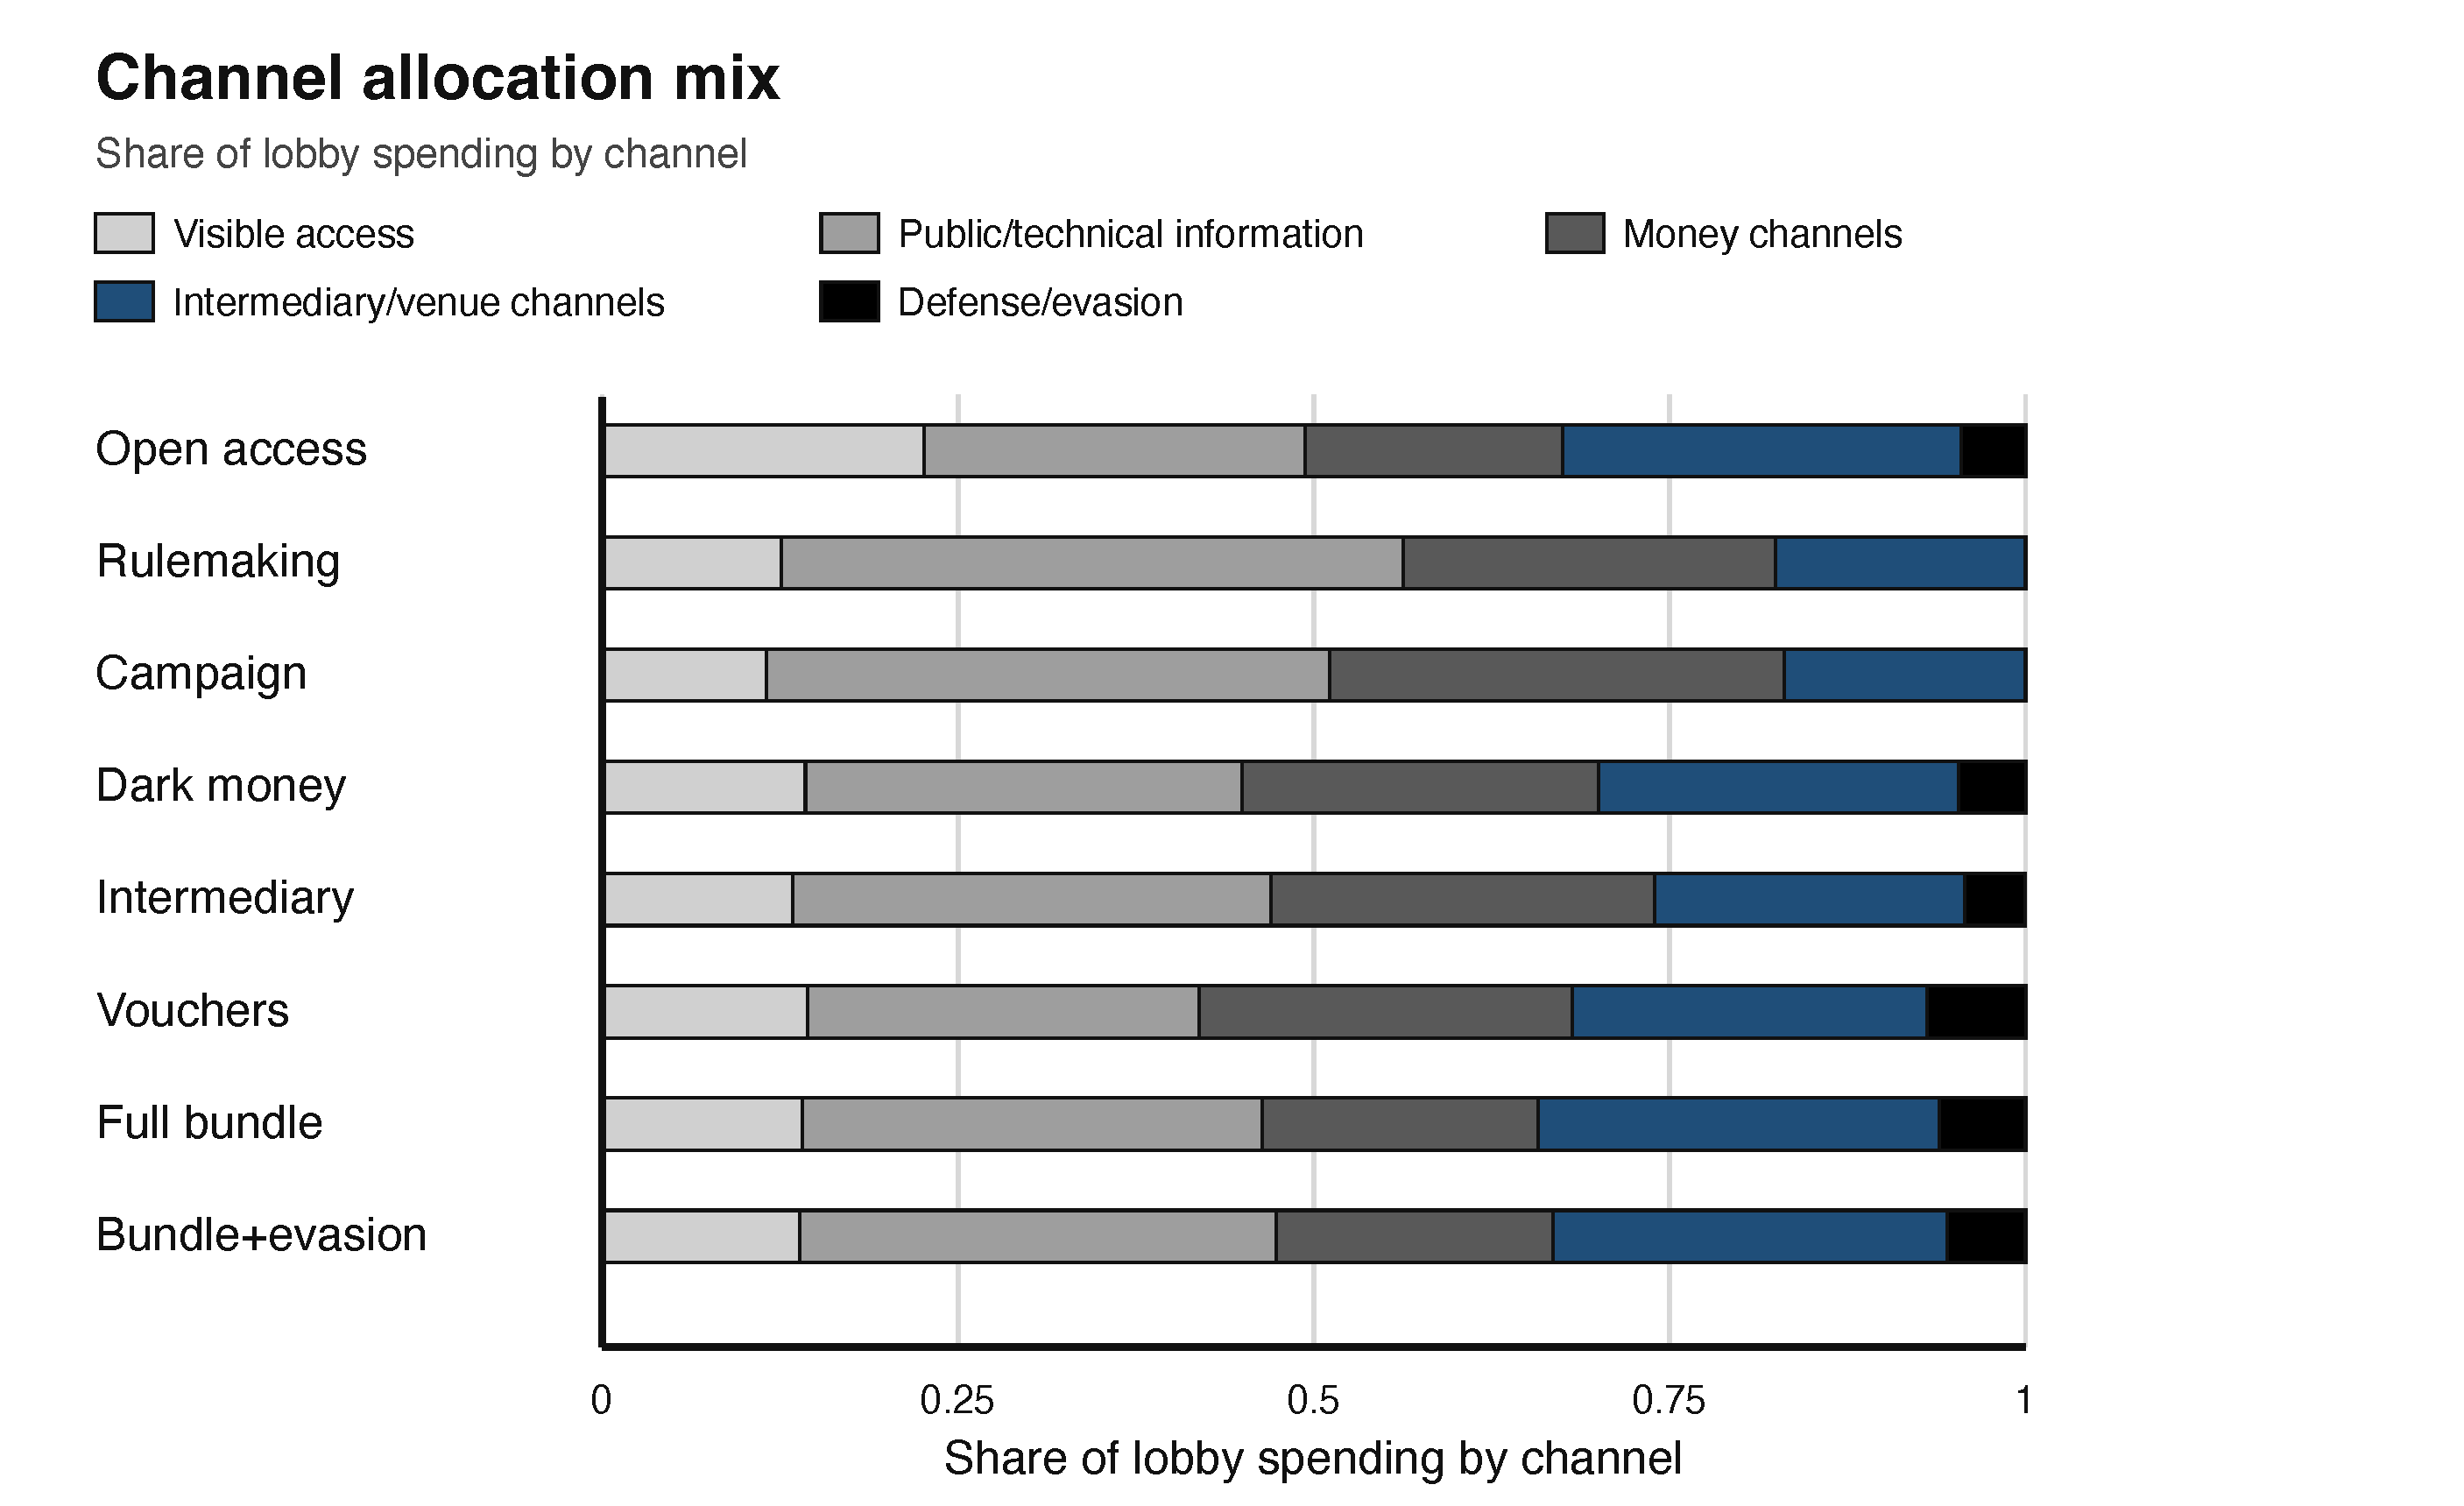
\includegraphics[width=0.82\linewidth]{figures/Figure_1_channel_mix.pdf}
\caption{Channel allocation mix for selected scenarios. The stacked bars show how the model routes lobbying budgets across access, information, public campaigns, campaign finance, dark money, revolving-door pressure, and defensive reform spending.}
\label{fig:channel-mix}
\end{figure}


% Generated by scripts/generate-interaction-figures.py; source=reports/lobby-capture-campaign.csv; graphic=Figure_4_scenario_tradeoffs.pdf; x=capture rate; y=Total influence distortion
\begin{figure}[htbp]
\centering
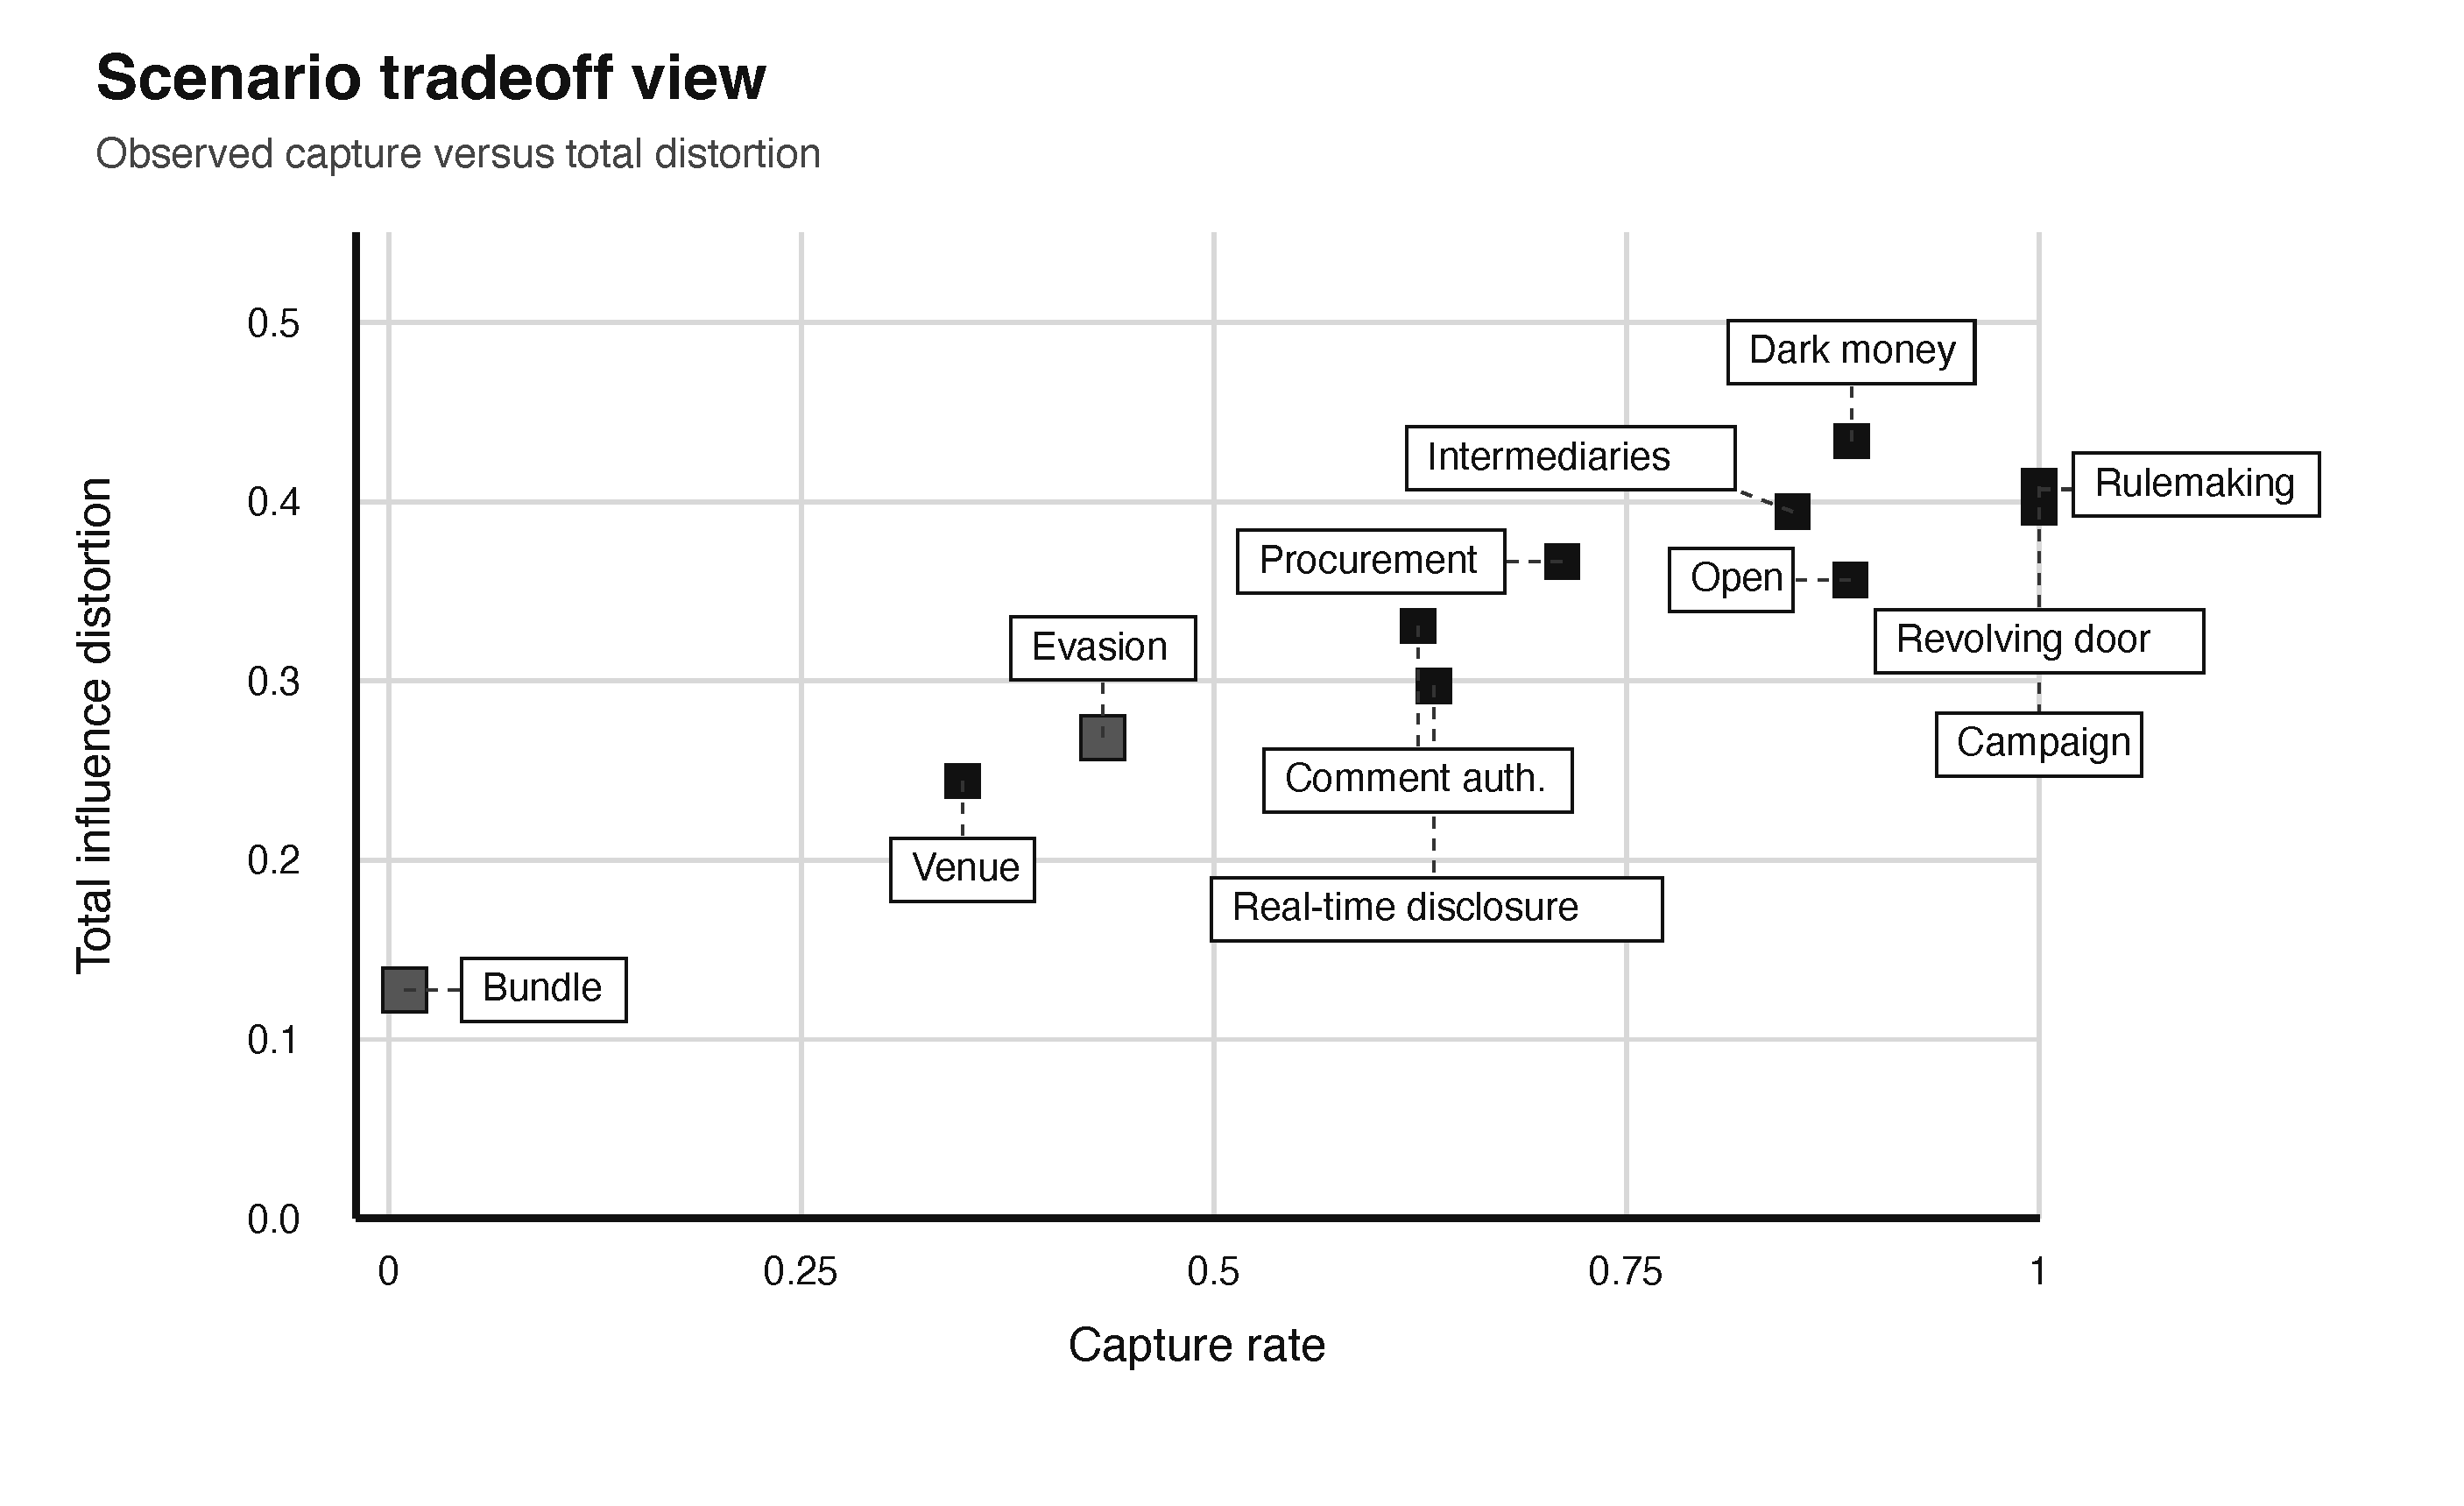
\includegraphics[width=0.76\linewidth]{figures/Figure_4_scenario_tradeoffs.pdf}
\caption{Scenario tradeoff between observed capture and total influence distortion across selected campaign scenarios.}
\label{fig:scenario-tradeoffs}
\end{figure}


The scenario rows also separate stress tests from ordinary interpretation. Open access, dark-money dominance, and intermediary dominance are not presented as estimates of national capture frequency. They are high-pressure worlds used to verify that the simulator can express recognizable failure modes. The full bundle and evasion-bundle contrast is more central. When evasion is constrained, the model reports low observed capture and lower distortion; when evasion is available, hidden influence and total distortion rebound. That contrast is the governance lesson: bundles that combine disclosure, enforcement, public participation, and venue detection perform differently from bundles that close visible channels but leave actors able to route influence through opaque money, intermediaries, or substitute venues.

The channel-mix figure is best read alongside the scenario table. Visible access does not disappear from the model; it becomes one option among money, technical information, public mobilization, intermediaries, litigation, procurement, and defensive spending. The result is a trace of influence movement rather than a claim that any one channel is always dominant. In some scenarios, procurement and technical information carry more diagnostic weight than campaign finance. In others, dark money and intermediaries preserve influence after formal disclosure improves. A regulatory-governance audience should read these rows as design stress tests for measurement systems: if the only available monitoring data are registered lobbying totals, the model intentionally withholds the most important movement.

\section{Substitution Warning Ranking}

Table~\ref{tab:apparent-failures} reports apparent-success distortion failures: cases where observed capture falls while total distortion rises. Table~\ref{tab:substitution-warnings} separately reports substitution-risk warnings, where hidden influence, substitution risk, or visible-channel movement worsens without meeting the stricter distortion-failure criterion. Figure~\ref{fig:substitution-warning-map} maps observed-capture change against total-distortion change relative to the comparison row.

% Generated by scripts/generate-paper-tables.py; source=reports/substitution-audit.csv; config=paper/tables.yml
\begingroup
\begin{center}
\begin{minipage}{\textwidth}
\centering
\scriptsize
\setlength{\tabcolsep}{1.5pt}
\begin{tabular*}{\textwidth}{@{\extracolsep{\fill}}lrrrrrrrr@{}}
\toprule
Report & Scenario & Status & Warn. score & Loss & Cap. delta & Hid. delta & Dist. delta & Risk delta \\
\midrule
Campaign & Ban+DM leakage & distortion fail & 1.289 & 0.333 & -0.2206 & +0.5831 & +0.0447 & +0.2391 \\
Campaign & Proc. mods & distortion fail & 1.009 & 0.291 & -0.2162 & +0.4175 & +0.0478 & +0.1714 \\
Campaign & Meeting-log leak & distortion fail & 0.841 & 0.239 & -0.2050 & +0.3568 & +0.0222 & +0.1315 \\
Campaign & Budget cap stress & distortion fail & 0.840 & 0.297 & -0.1731 & +0.3686 & +0.0211 & +0.1558 \\
Campaign & Intermediaries & distortion fail & 0.527 & 0.233 & -0.0350 & +0.2704 & +0.0381 & +0.1002 \\
\bottomrule
\end{tabular*}
\par\smallskip
\captionsetup{hypcap=false}
\captionof{table}{Apparent-success distortion failures. Rows have lower observed capture and higher total modeled distortion relative to the comparison row.}
\label{tab:apparent-failures}
\end{minipage}
\end{center}
\endgroup


% Generated by scripts/generate-paper-tables.py; source=reports/substitution-audit.csv; config=paper/tables.yml
\begingroup
\begin{center}
\begin{minipage}{\textwidth}
\centering
\scriptsize
\setlength{\tabcolsep}{1.5pt}
\begin{tabular*}{\textwidth}{@{\extracolsep{\fill}}lrrrrrrrr@{}}
\toprule
Report & Scenario & Status & Warn. score & Loss & Cap. delta & Hid. delta & Dist. delta & Risk delta \\
\midrule
Campaign & Shadow max & subst. warn. & 1.188 & 0.309 & -0.3175 & +0.4853 & +0.0125 & +0.1986 \\
Campaign & Opaque network substitution frontier & subst. warn. & 1.103 & 0.239 & -0.3162 & +0.4673 & -0.0102 & +0.1670 \\
Campaign & Bundle+evasion & subst. warn. & 0.949 & 0.209 & -0.4528 & +0.3024 & -0.0879 & +0.1126 \\
Campaign & Public-finance dark-money frontier & subst. warn. & 0.948 & 0.241 & -0.3915 & +0.3130 & -0.0536 & +0.1410 \\
Campaign & Full bundle & subst. warn. & 0.910 & 0.118 & -0.8762 & +0.0334 & -0.2287 & -0.0165 \\
Campaign & Comment tech subst. & subst. warn. & 0.879 & 0.288 & -0.2487 & +0.3511 & +0.0033 & +0.1553 \\
Campaign & Public finance/IE & subst. warn. & 0.817 & 0.267 & -0.2268 & +0.3124 & +0.0097 & +0.1553 \\
Campaign & Procurement shift & subst. warn. & 0.799 & 0.263 & -0.2525 & +0.2982 & +0.0126 & +0.1243 \\
\bottomrule
\end{tabular*}
\par\smallskip
\captionsetup{hypcap=false}
\captionof{table}{Substitution-risk warnings. Rows are not apparent-success distortion failures but show higher hidden influence, substitution risk, or visible-channel movement relative to the comparison row.}
\label{tab:substitution-warnings}
\end{minipage}
\end{center}
\endgroup


% Generated by scripts/generate-interaction-figures.py; source=reports/substitution-audit.csv; graphic=Figure_5_substitution_warning_map.pdf; x=observed capture change versus comparison; y=total distortion change versus comparison
\begin{figure}[tbp]
\centering
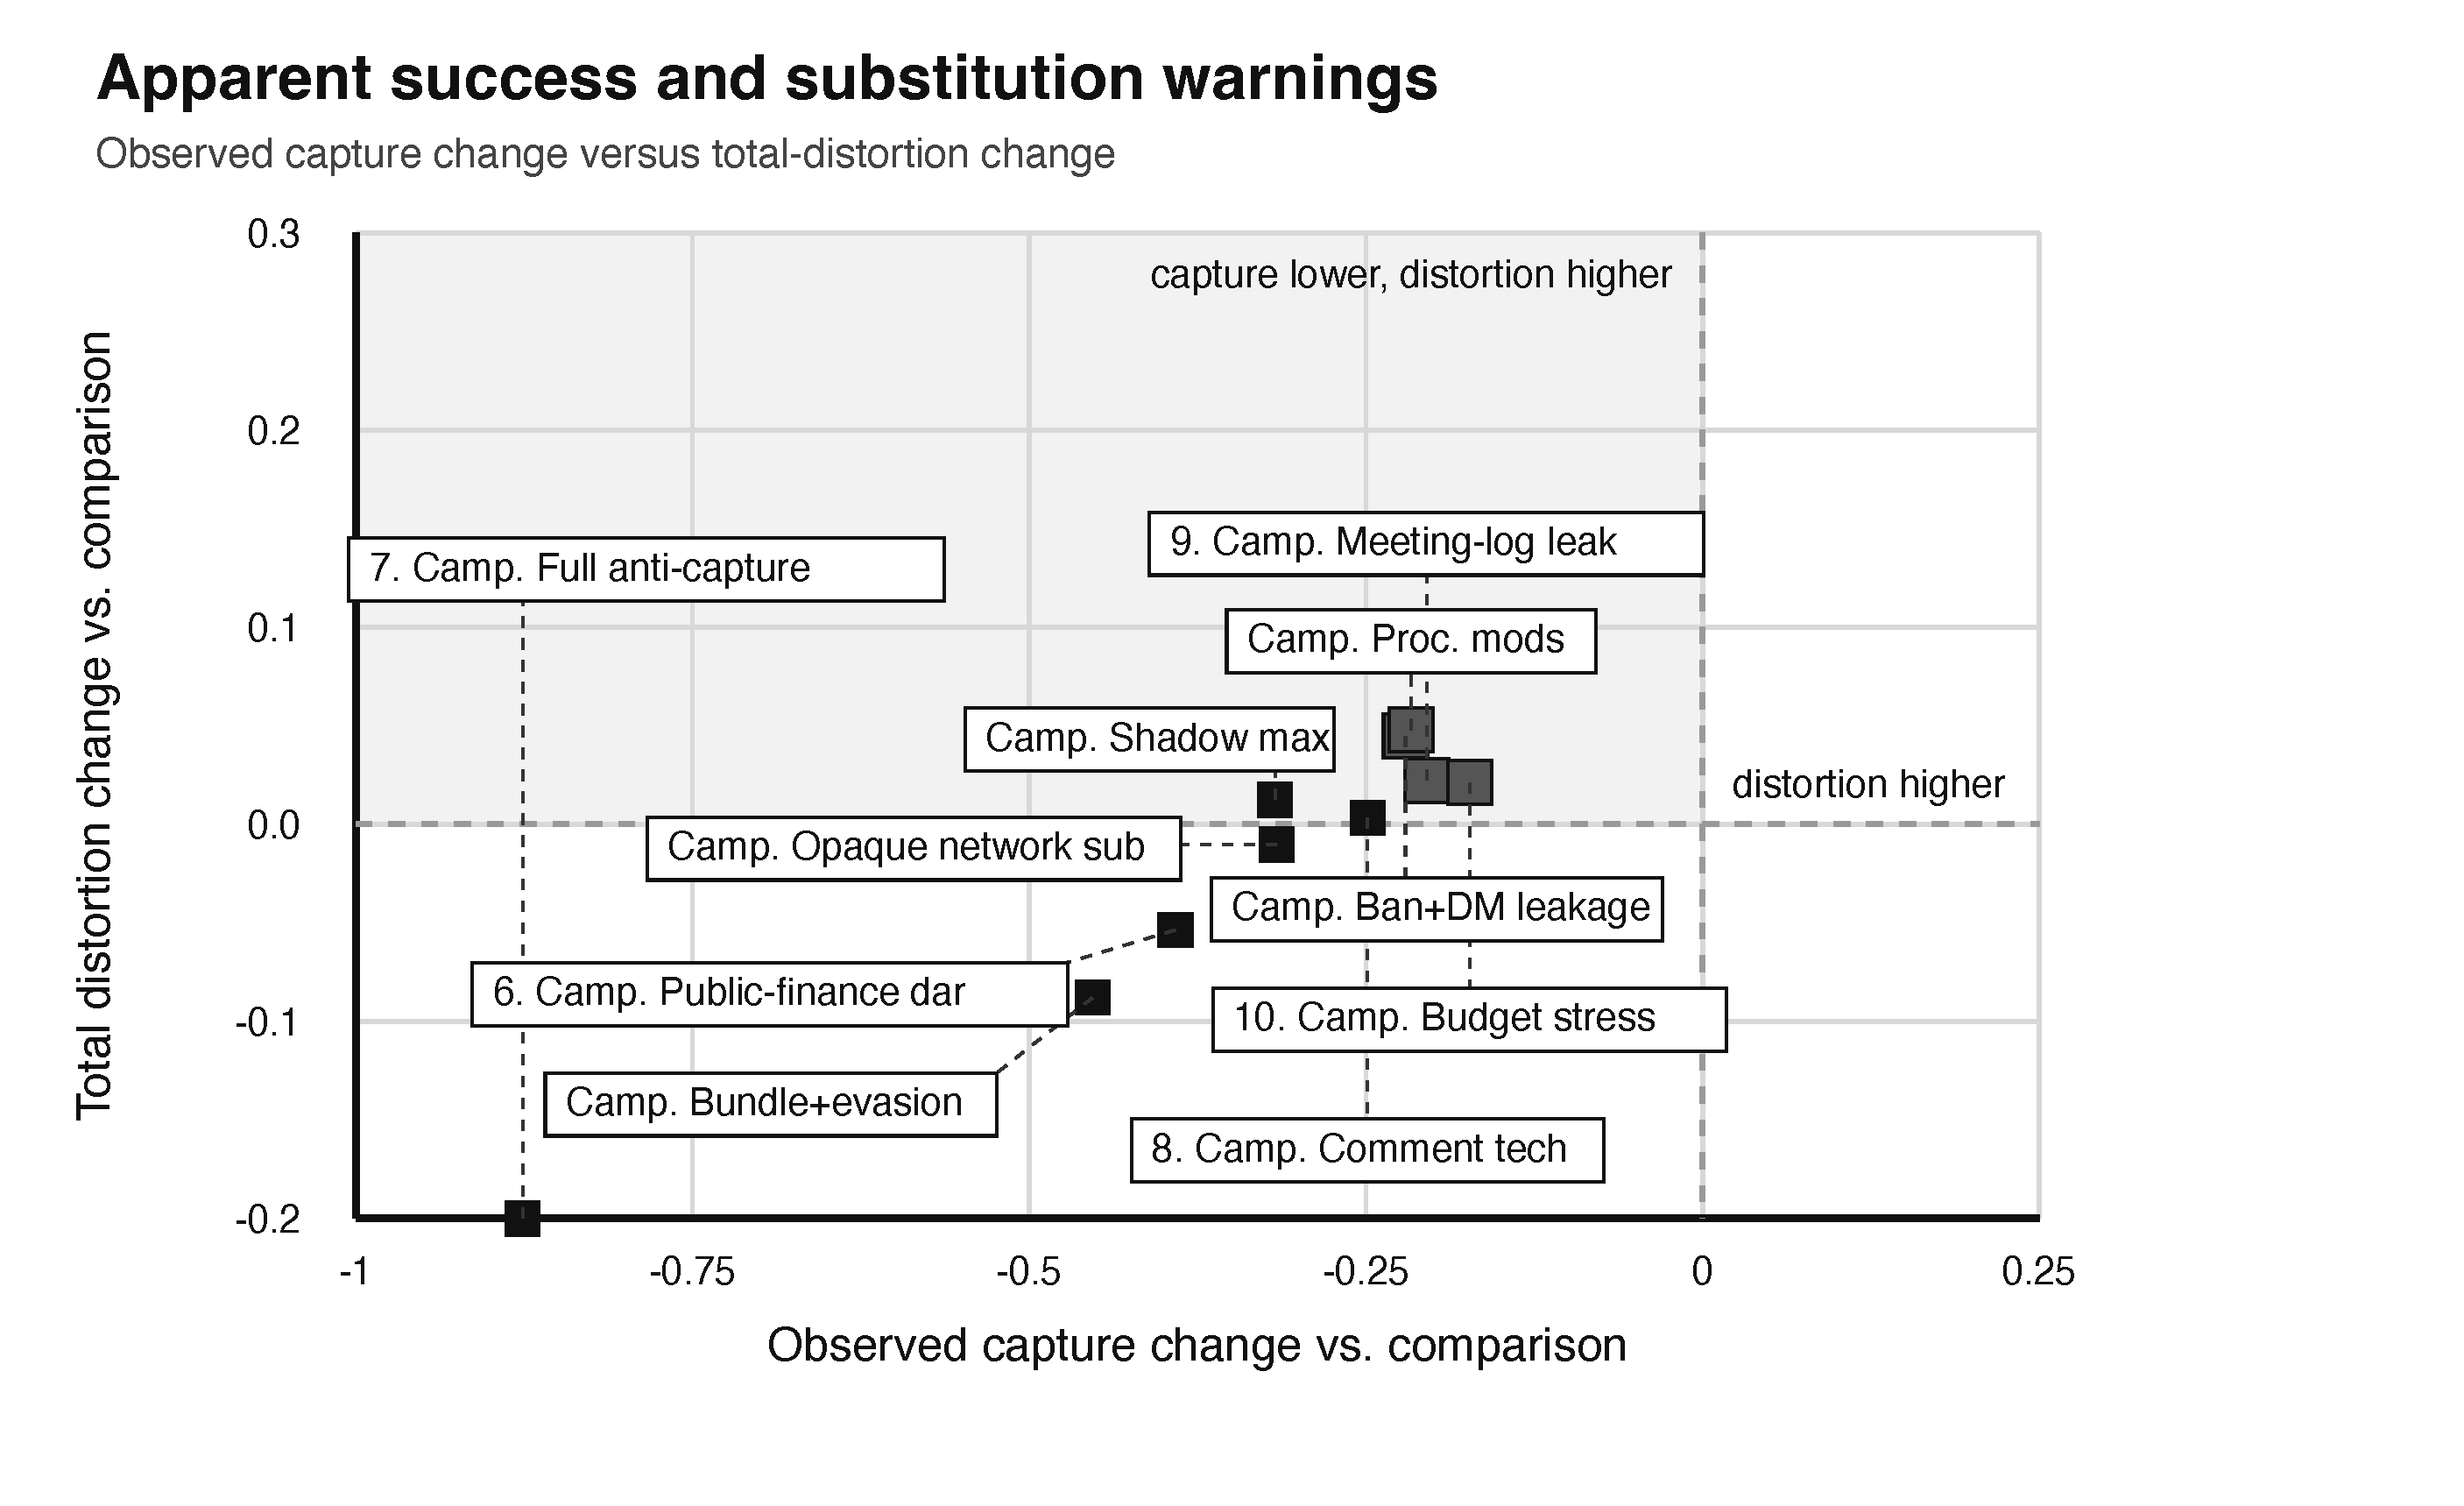
\includegraphics[width=0.82\linewidth]{figures/Figure_5_substitution_warning_map.pdf}
\caption{Substitution-warning map. The shaded upper-left quadrant combines lower observed capture with higher total influence distortion. Other points are warnings where hidden influence, hidden capture, or substitution risk rises even if total distortion does not.}
\label{fig:substitution-warning-map}
\end{figure}


\section{Sensitivity Snapshot}

The sensitivity sweep varies enforcement, disclosure, public financing, cooling-off, and evasion freedom around the full anti-capture bundle. Table~\ref{tab:sensitivity} shows selected low- and high-leverage settings.

% Generated by scripts/generate-paper-tables.py; source=reports/lobby-capture-sensitivity.csv; config=paper/tables.yml; reportGeneratedAt=2026-05-05T00:00:00Z; seed=142; runs=30; contestsPerRun=70
\begingroup
\begin{center}
\begin{minipage}{\textwidth}
\centering
\footnotesize
\setlength{\tabcolsep}{3pt}
\begin{tabular*}{\textwidth}{@{\extracolsep{\fill}}lrrrrrr@{}}
\toprule
Scenario & Capture & Cap. SD & Total dist. & Hidden cap. & Subst. risk & Dist. SD \\
\midrule
Enforcement 0.10 & 0.391 & 0.054 & 0.2503 & 0.1055 & 0.2101 & 0.0184 \\
Disclosure 0.10 & 0.635 & 0.063 & 0.3285 & 0.1345 & 0.2622 & 0.0213 \\
Public financing 1.25 & 0.098 & 0.034 & 0.1666 & 0.0731 & 0.1642 & 0.0109 \\
Public financing 0.35 & 0.124 & 0.045 & 0.1703 & 0.0708 & 0.1577 & 0.0153 \\
Evasion 0.00 & 0.018 & 0.015 & 0.1211 & 0.0351 & 0.1006 & 0.0067 \\
Evasion 0.60 & 0.250 & 0.055 & 0.2237 & 0.1112 & 0.2203 & 0.0203 \\
Evasion 0.90 & 0.565 & 0.066 & 0.3260 & 0.1853 & 0.3138 & 0.0260 \\
\bottomrule
\end{tabular*}
\par\smallskip
\captionsetup{hypcap=false}
\captionof{table}{Selected sensitivity sweep rows. Rows report capture, total distortion, hidden capture, substitution risk, and run-level standard deviations.}
\label{tab:sensitivity}
\end{minipage}
\end{center}
\endgroup


Figure~\ref{fig:evasion-sensitivity} isolates the evasion slice from the sensitivity table. Stronger evasion freedom preserves hidden influence and raises total distortion in this scenario family.

% Generated by scripts/generate-interaction-figures.py; source=reports/lobby-capture-sensitivity.csv; graphic=Figure_2_evasion_sensitivity.pdf
\begin{figure}[tbp]
\centering
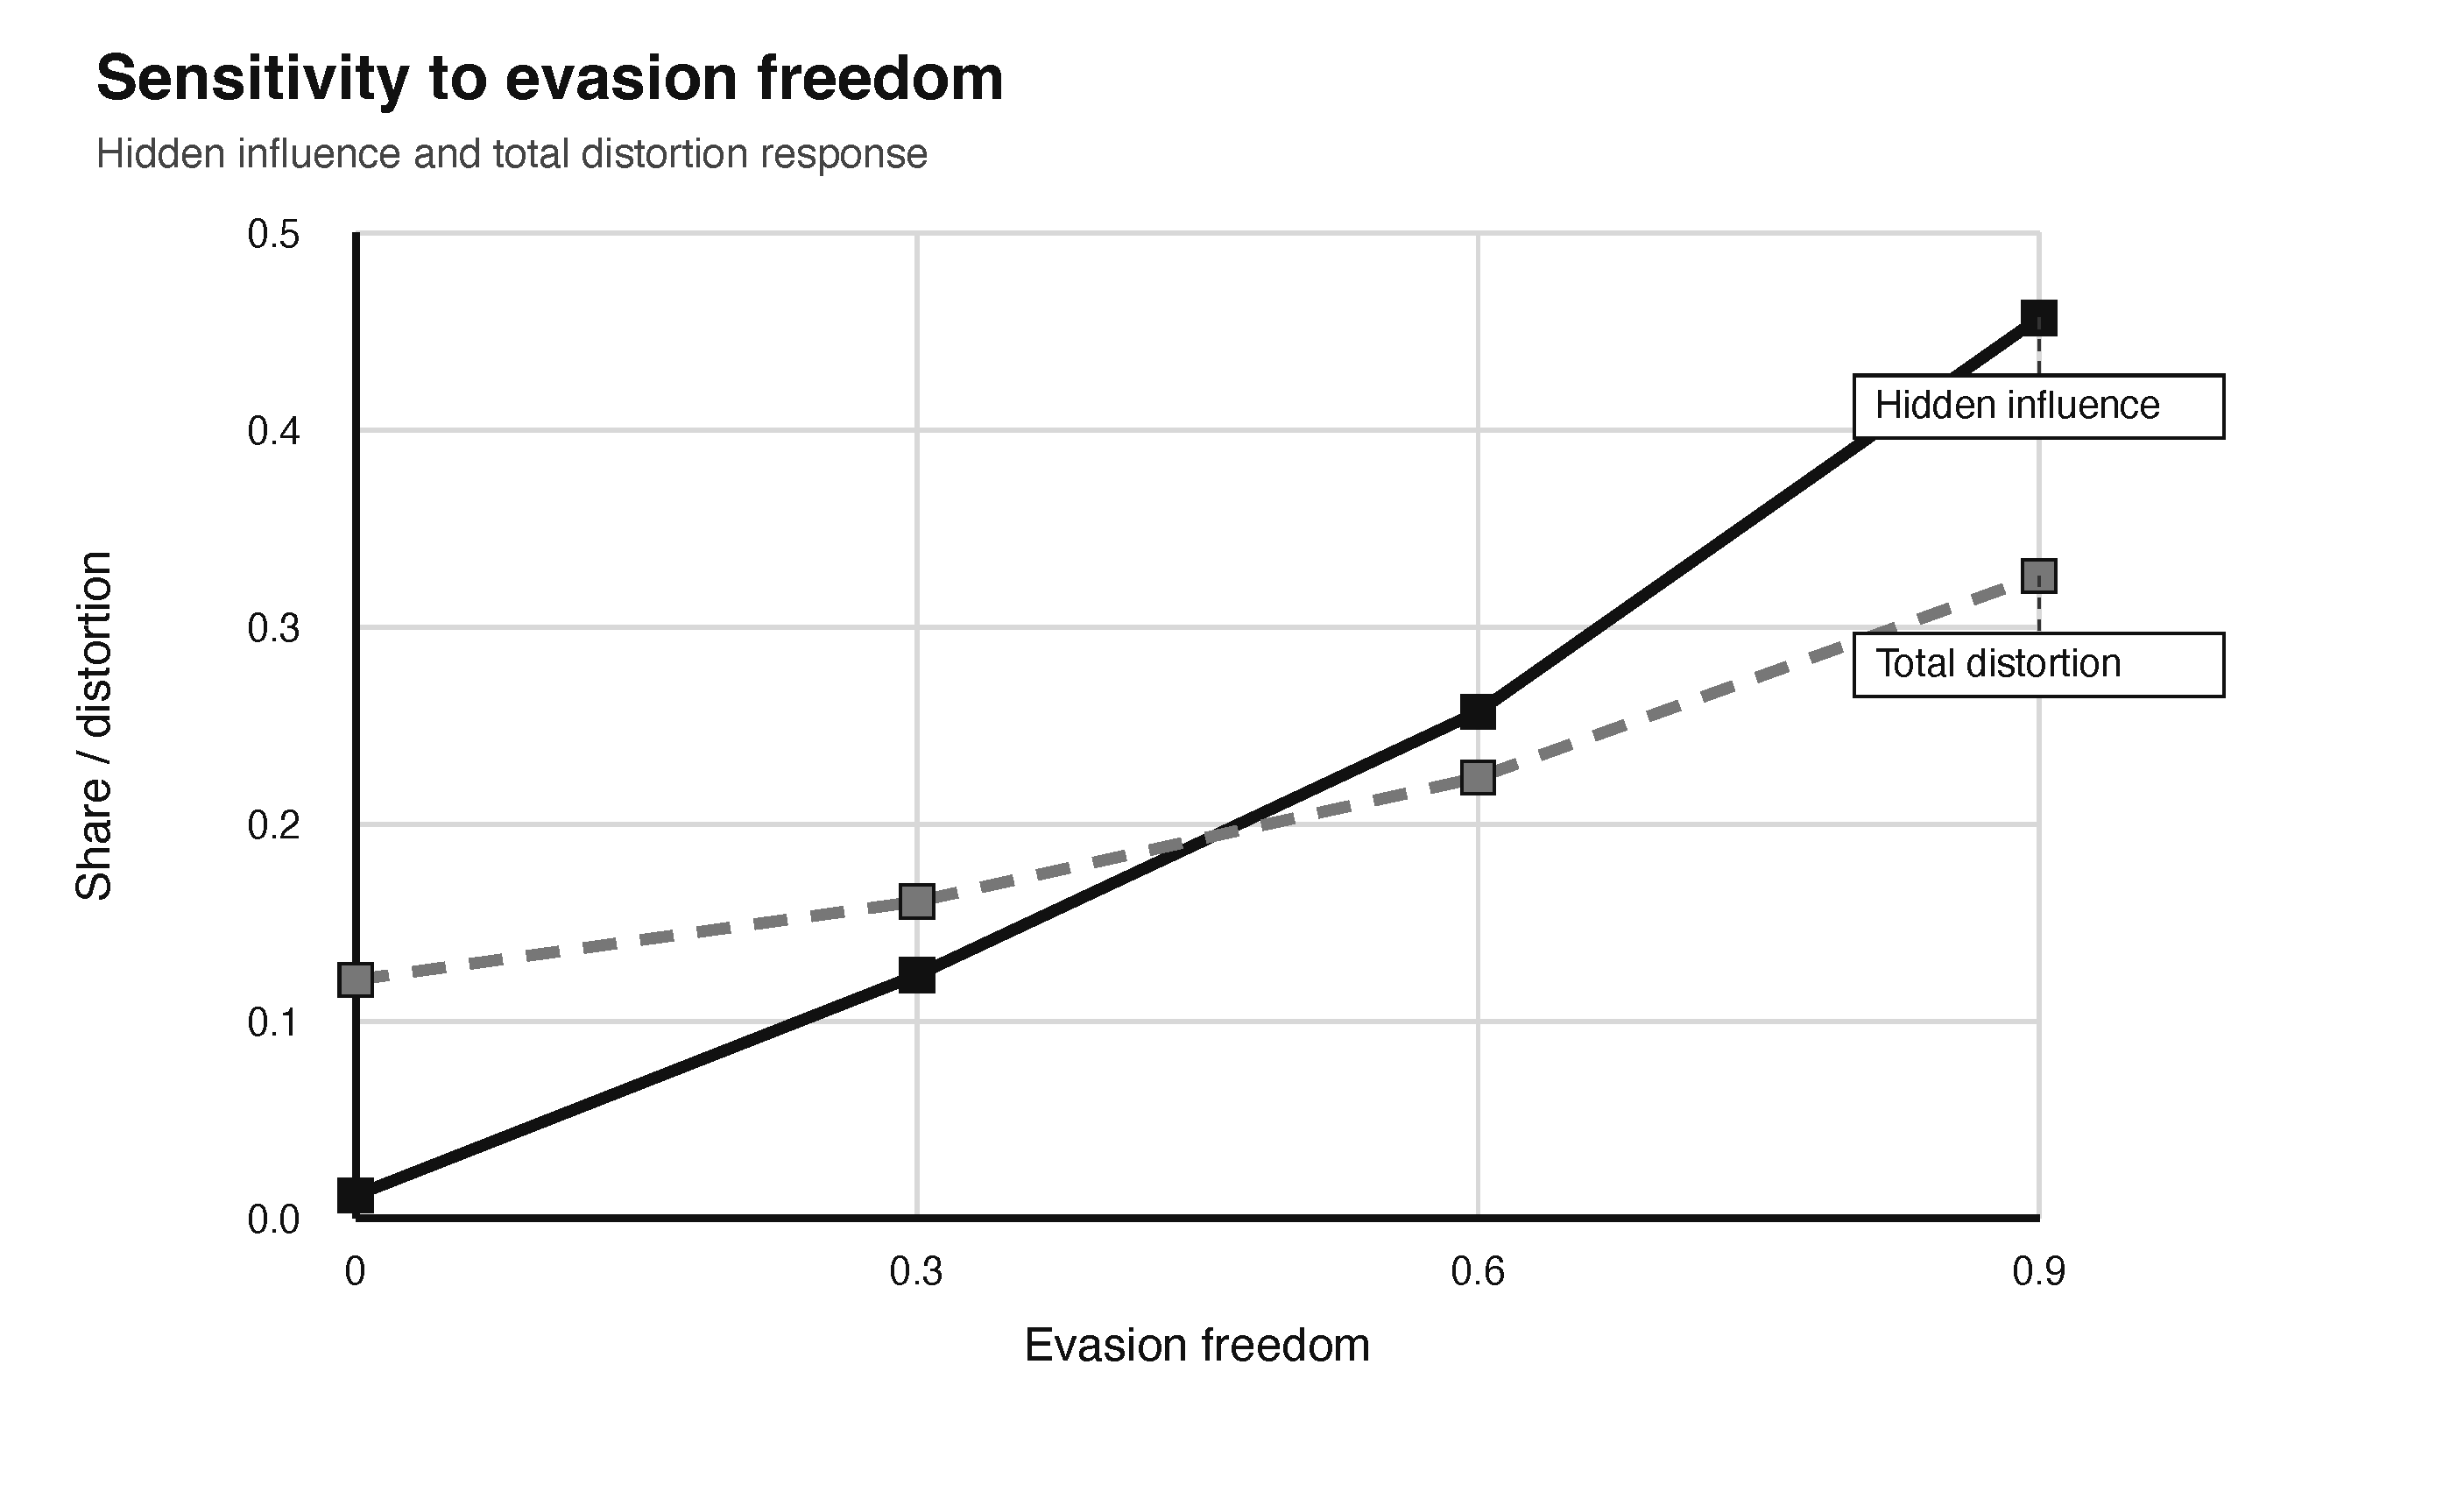
\includegraphics[width=0.82\linewidth]{figures/Figure_2_evasion_sensitivity.pdf}
\caption{Sensitivity to evasion freedom. The figure plots hidden influence and total influence distortion across evasion-freedom settings.}
\label{fig:evasion-sensitivity}
\end{figure}


This is the cleanest mechanism check in the results because only one strategic capacity is moving. At low evasion freedom, the reform bundle suppresses capture and keeps hidden capture low. As evasion freedom rises, observed capture, total distortion, hidden capture, and substitution risk rise together. The point is not that evasion freedom has this exact slope in the real world. The point is that anti-capture systems need to specify what makes evasion costly: beneficial-owner disclosure, meeting-log coverage, audit probability, cross-venue entity resolution, sanctions, procurement firewalls, and comment-authenticity rules. If those controls are weak, visible-channel restrictions can create a misleading compliance surface.

The sensitivity results also discipline the portfolio interpretation. Public financing alone does not eliminate capture in every scenario, and stronger disclosure alone is not enough when enforcement is weak. The model rewards combinations that reduce the return to substitution, not symbolic breadth. In governance terms, a reform bundle should make hidden routing less profitable, increase the chance of cross-venue detection, and preserve legitimate participation so that organized interests do not become the only actors able to absorb procedural costs.

\section{Ablation Snapshot}

Ablation reporting removes one reform component from the full anti-capture bundle. Table~\ref{tab:ablation} measures each distortion change against the full-bundle baseline in the same stress-test family.

% Generated by scripts/generate-paper-tables.py; source=reports/lobby-capture-ablation.csv; config=paper/tables.yml; reportGeneratedAt=2026-05-05T00:00:00Z; seed=242; runs=40; contestsPerRun=80
\begingroup
\begin{center}
\begin{minipage}{\textwidth}
\centering
\footnotesize
\setlength{\tabcolsep}{3pt}
\begin{tabular*}{\textwidth}{@{\extracolsep{\fill}}lrrrrr@{}}
\toprule
Removed component & Total-dist. change & Capture change & Hidden cap. & Subst. risk & Comment flood \\
\midrule
Beneficial-owner disclosure & 0.1203 & 0.3747 & 0.0584 & 0.2539 & 0.2163 \\
Enforcement & 0.0892 & 0.3312 & 0.0343 & 0.2125 & 0.2176 \\
Public advocate/blind review & 0.0451 & 0.1956 & -0.0047 & 0.1524 & 0.2490 \\
Public financing/vouchers & 0.0064 & 0.0322 & -0.0004 & 0.1603 & 0.2193 \\
Anti-astroturf authentication & -0.0024 & 0.0115 & -0.0093 & 0.1498 & 0.2424 \\
Cooling-off rules & -0.0073 & -0.0075 & -0.0069 & 0.1506 & 0.2197 \\
\bottomrule
\end{tabular*}
\par\smallskip
\captionsetup{hypcap=false}
\captionof{table}{Selected ablation results. Removals are ranked by total-distortion change relative to the full-bundle baseline.}
\label{tab:ablation}
\end{minipage}
\end{center}
\endgroup


Negative ablation deltas should not be read as evidence that the removed reform is harmful in general. They indicate that, under this contest mix and weighting scheme, the administrative or substitution costs of that component can exceed its modeled reduction in distortion.

\section{Interaction Snapshot}

The interaction sweep varies enforcement, disclosure, public financing, evasion freedom, cooling-off rules, and revolving-door strategy. Table~\ref{tab:interactions} shows selected combinations that separate nominal reform strength from substitution response. A reform can lower visible pressure while preserving influence through hidden messengers, intermediaries, or alternate venues.

% Generated by scripts/generate-paper-tables.py; source=reports/lobby-capture-interactions.csv; config=paper/tables.yml; reportGeneratedAt=2026-05-05T00:00:00Z; seed=342; runs=25; contestsPerRun=60
\begin{table*}[tbp]
\centering
\scriptsize
\setlength{\tabcolsep}{3pt}
\begin{tabular*}{\textwidth}{@{\extracolsep{\fill}}lrrrrrrrr@{}}
\toprule
Scenario & Cap. (95\% CI) & Dist. & Hid. cap. & Risk & Hidden & Venue & Intermed. & Admin \\
\midrule
Low E/D & 0.715 [0.691, 0.737] & 0.365 & 0.162 & 0.302 & 0.317 & 0.177 & 0.088 & 0.470 \\
High E/D & 0.018 [0.012, 0.026] & 0.141 & 0.067 & 0.148 & 0.133 & 0.049 & 0.134 & 0.617 \\
High finance/evasion & 0.627 [0.603, 0.651] & 0.351 & 0.209 & 0.345 & 0.513 & 0.211 & 0.129 & 0.638 \\
High cooling/RD & 0.137 [0.121, 0.156] & 0.182 & 0.085 & 0.183 & 0.177 & 0.086 & 0.133 & 0.615 \\
\bottomrule
\end{tabular*}
\caption{Selected reform-interaction rows under the stressed contest mix. The table reports capture with Wilson intervals alongside total-distortion and substitution diagnostics.}
\label{tab:interactions}
\end{table*}


Figure~\ref{fig:interaction-tradeoffs} presents the same interaction slice as a tradeoff view, with hidden influence on one axis and total distortion on the other.

% Generated by scripts/generate-interaction-figures.py; source=reports/lobby-capture-interactions.csv; graphic=Figure_3_interaction_tradeoffs.pdf; x=hidden influence; y=Total influence distortion
\begin{figure}[tbp]
\centering
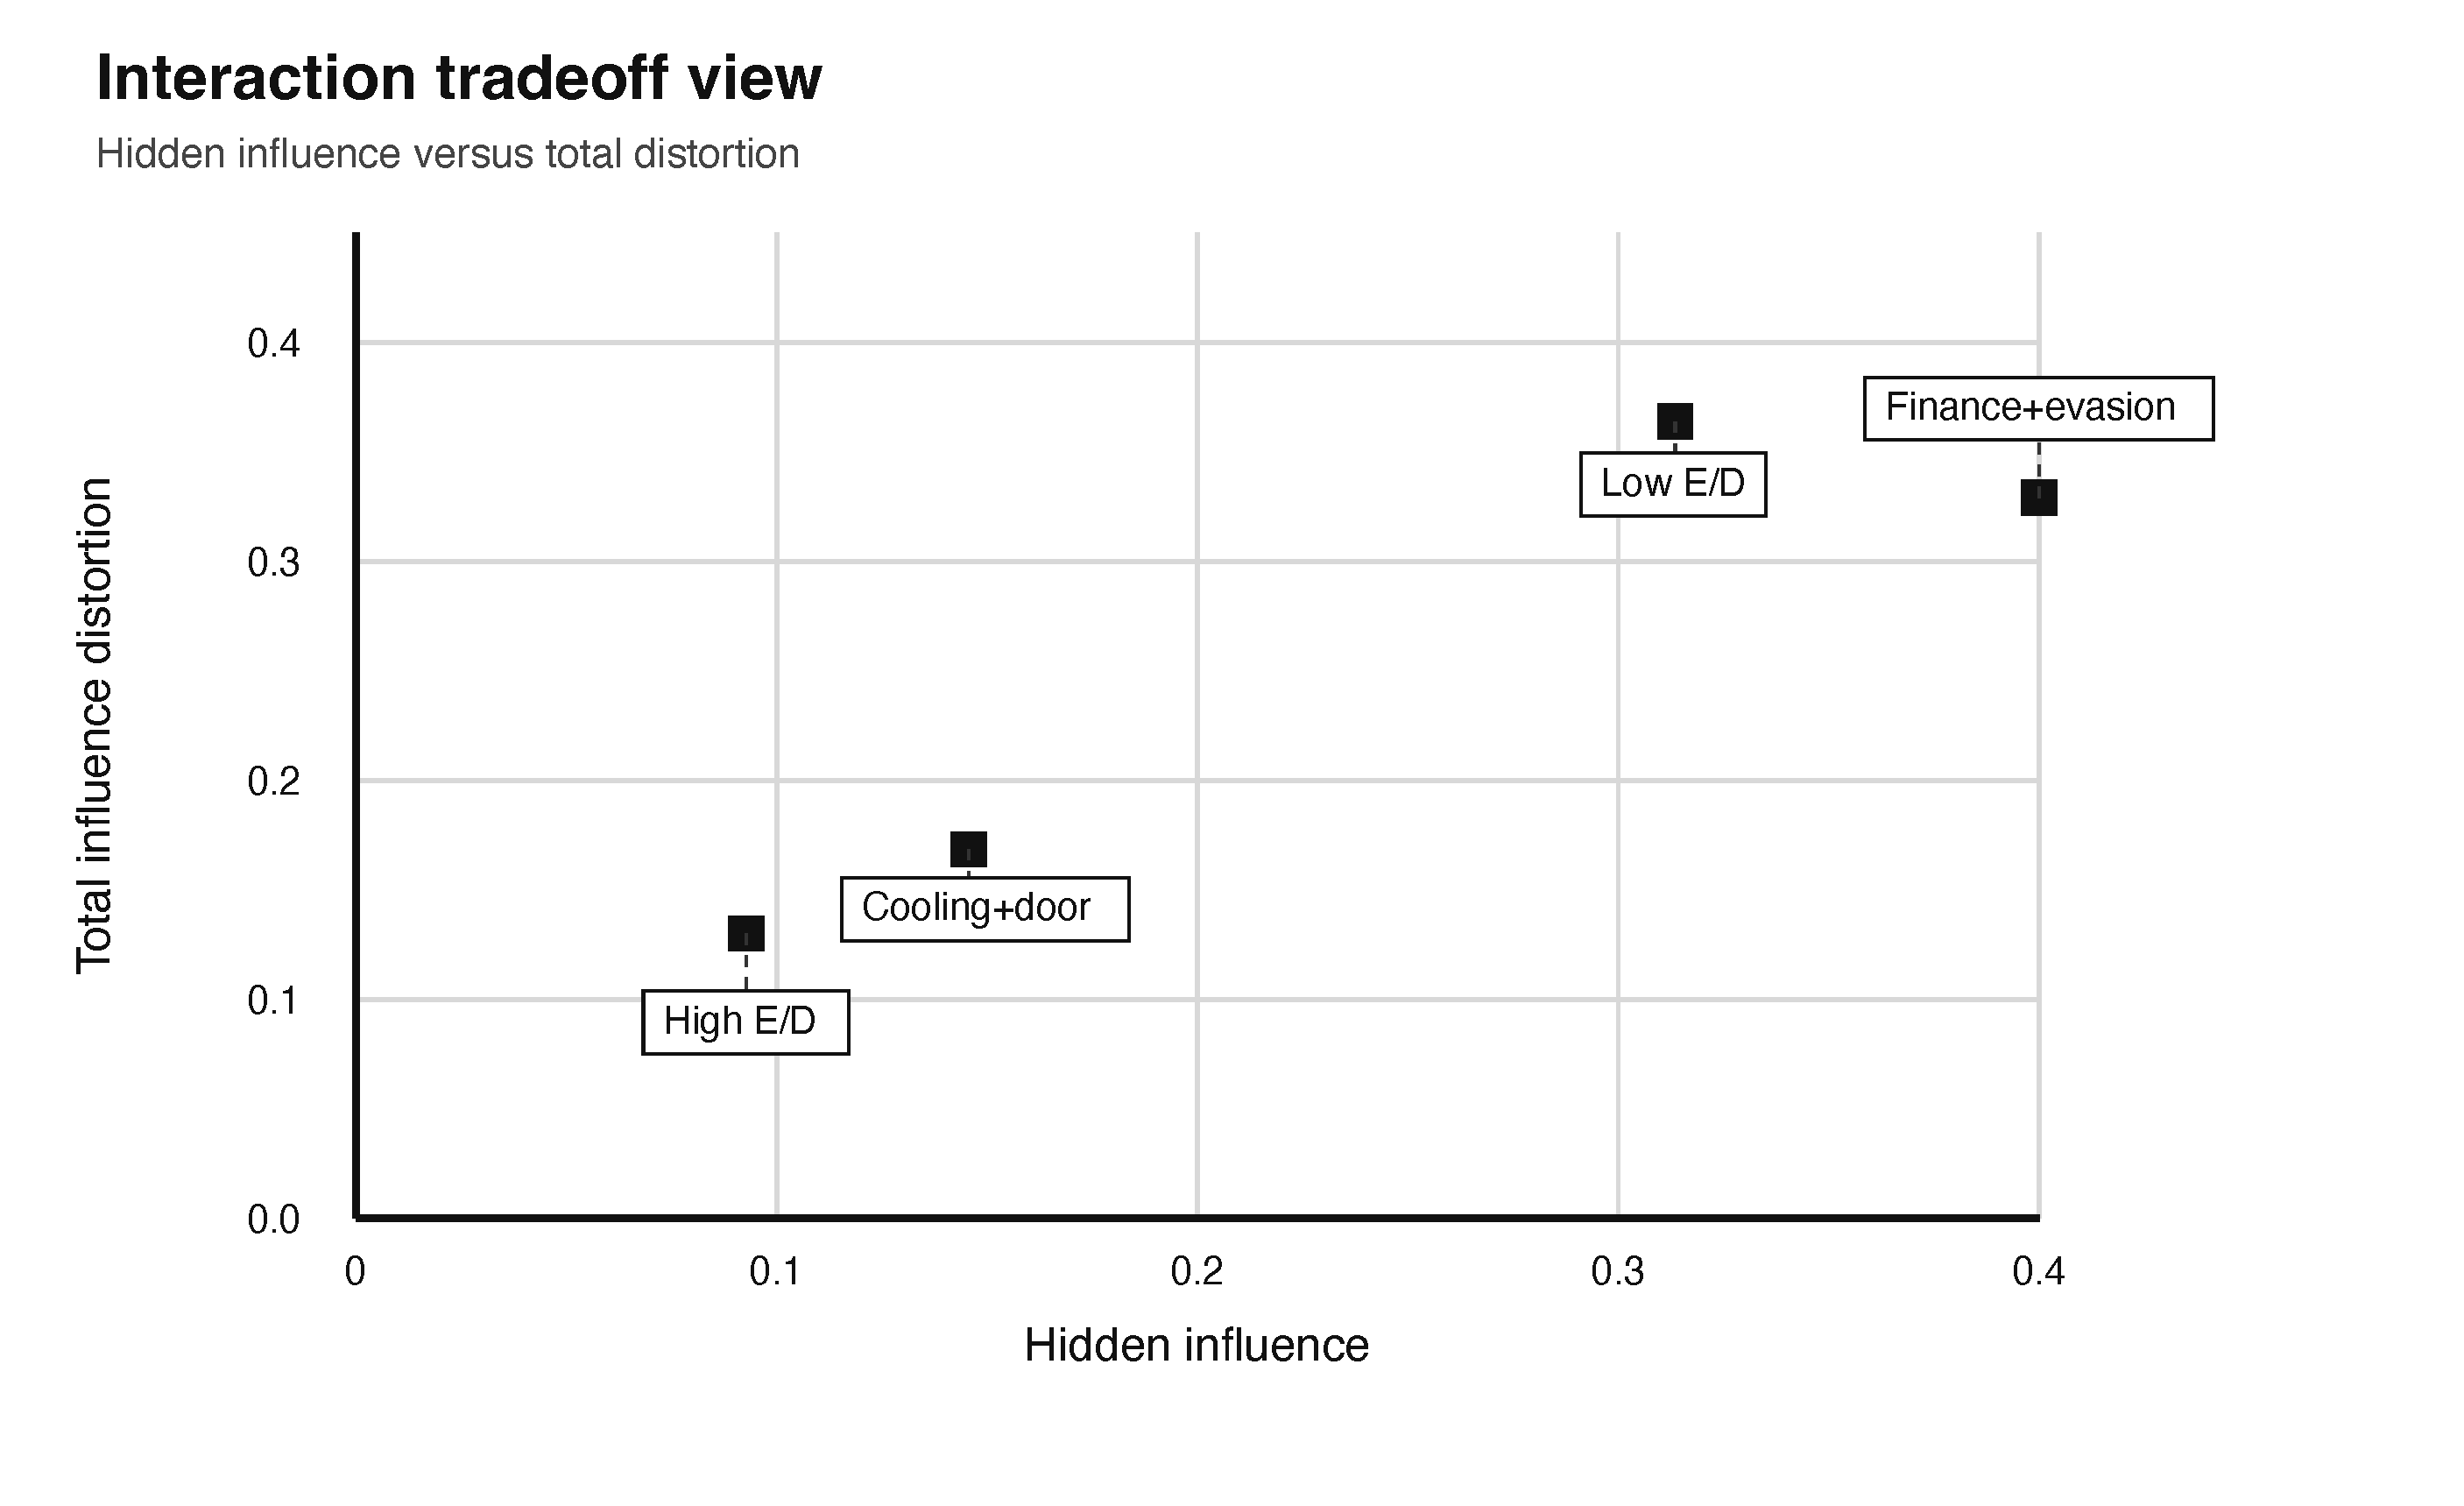
\includegraphics[width=0.82\linewidth]{figures/Figure_3_interaction_tradeoffs.pdf}
\caption{Interaction tradeoff view. Points compare hidden influence against total influence distortion after reforms bind.}
\label{fig:interaction-tradeoffs}
\end{figure}


\section{Portfolio Screen}

The portfolio screen compares transparency, balanced compliance, electoral shielding, rulemaking integrity, procurement hardening, countervailing representation, high-deterrence enforcement, civil-liberties-constrained enforcement, and full anti-substitution designs. The criterion minimizes total influence distortion first, then hidden capture, substitution risk, administrative burden, network opacity, legitimate-advocacy chill, and speech-restriction risk, while rewarding cross-venue detection and participation protection. Because those weights are normative, the screen should be read as a design diagnostic rather than a policy ranking.

% Generated by scripts/generate-paper-tables.py; source=reports/lobby-capture-portfolio.csv; config=paper/tables.yml; reportGeneratedAt=2026-05-05T00:00:00Z; seed=442; runs=35; contestsPerRun=70
\begin{table*}[tbp]
\centering
\scriptsize
\setlength{\tabcolsep}{3pt}
\begin{tabular*}{\textwidth}{@{\extracolsep{\fill}}lrrrrrrrr@{}}
\toprule
Portfolio & Capture & Dist. & Hid. cap. & Subst. & Venue det. & Opacity & Chill & Admin \\
\midrule
Transparency & 0.640 & 0.309 & 0.100 & 0.192 & 0.579 & 0.351 & 0.076 & 0.270 \\
Balanced & 0.473 & 0.269 & 0.098 & 0.195 & 0.643 & 0.379 & 0.137 & 0.411 \\
Electoral shield & 0.607 & 0.312 & 0.118 & 0.226 & 0.616 & 0.449 & 0.079 & 0.454 \\
Rulemaking & 0.485 & 0.283 & 0.121 & 0.232 & 0.562 & 0.430 & 0.168 & 0.484 \\
Procurement & 0.367 & 0.245 & 0.096 & 0.196 & 0.679 & 0.371 & 0.139 & 0.550 \\
Countervailing & 0.491 & 0.279 & 0.106 & 0.216 & 0.421 & 0.477 & 0.036 & 0.395 \\
Civil-liberties & 0.284 & 0.223 & 0.095 & 0.194 & 0.705 & 0.312 & 0.074 & 0.426 \\
Full anti-sub. & 0.067 & 0.157 & 0.076 & 0.168 & 0.822 & 0.245 & 0.140 & 0.560 \\
Full+evasion & 0.566 & 0.334 & 0.201 & 0.333 & 0.822 & 0.330 & 0.145 & 0.585 \\
\bottomrule
\end{tabular*}
\caption{Portfolio screen under the stressed contest mix. Rows are candidate design bundles; the table reports total distortion, hidden capture, substitution risk, cross-venue detection, network opacity, legitimate-advocacy chill, and administrative burden so the preferred portfolio is not chosen by visible capture alone.}
\label{tab:portfolio}
\end{table*}


The comparison between the civil-liberties-constrained portfolio and the full anti-substitution portfolio illustrates the governance tradeoff. Full anti-substitution controls can reduce capture and distortion more strongly, while the civil-liberties design accepts higher modeled distortion in exchange for lower administrative burden, chill, or speech-restriction risk.

\section{Validation Plan}

Validation uses five layers: schema checks, source-moment checks, scenario diagnostics, validation-queue tracking, and a causal-calibration target matrix. These checks verify implementation consistency and identify empirical gaps; they do not estimate reform-effect magnitudes. The supporting information documents the detailed targets, artifacts, validation queues, and causal-calibration blockers \citep{ldaData,fecData,federalRegisterApi,regulationsGovApi,nycCfbData,seattleVouchers,irsEoBmf,usaspending}.

\section{Discussion}

The model-mode comparison shows what the single-channel baseline misses: reform diagnostics change once organized interests can move through alternative messengers, venues, financing routes, and intermediaries. Robust stress-test features pair visibility with enforcement capacity, countervailing representation, procurement safeguards, and cross-venue detection. The main failure modes are evasion freedom, opaque intermediary paths, defensive mobilization, and administrative burden that can weaken legitimate participation. Some strong-reform rows remain near saturated observed capture, so the clearest result is the substitution pattern conditional on that design.

\textbf{Implications for regulatory-governance design.} Channel-specific reforms can mislead when evaluation follows only the closed channel. Anti-capture systems need cross-venue detection because influence can move through adjacent institutional surfaces: campaign finance, dark money, intermediaries, procurement, comments, litigation, and revolving-door access. Countervailing participation and enforcement capacity matter because transparency can improve legibility without reducing total influence distortion when organized interests retain resources to substitute or delay.

This framing fits regulatory governance because the unit of analysis is a design problem across institutional venues. Transparency, countervailing participation, procedural integrity, enforcement budgets, procurement firewalls, and revolving-door controls operate as interacting features of one governance architecture. The policy-relevant output is a map of where influence moves when a rule binds.

The theoretical payoff is a shift from channel compliance to system resilience. A channel-compliance view asks whether a lobbying registration, donation report, comment docket, or procurement file satisfies the rule attached to that record. A system-resilience view asks whether the governance architecture still lets decision makers see who is trying to influence what, through whom, at what cost to public participation, and with what enforcement capacity. The model formalizes that distinction by making cross-venue movement an output rather than an anecdotal concern.

It also makes negative evidence useful. If a reform closes a channel and no adjacent pressure rises, that is evidence against the substitution assumption for that domain. If pressure rises in a venue the reform did not monitor, that is evidence that the governance system was under-instrumented.

Both outcomes are informative for institutional learning, comparative case selection, and future calibration.

For institutional design, the model suggests four questions that are more useful than asking whether a reform reduces one reported activity. First, what adjacent route becomes more attractive when the visible route is restricted? Second, does the reform increase the probability that money, messengers, vendors, docket comments, procurement records, and meetings can be linked across datasets? Third, does the reform add participation capacity for diffuse or public-interest actors, or does it mainly add compliance costs that concentrated interests can absorb? Fourth, does enforcement capacity scale with the new disclosure surface, or does the reform create more records than agencies can review?

Those questions change how familiar reforms are interpreted. Real-time meeting logs are not valuable only because they publish calendars; they are valuable when they can be linked to dockets, procurement actions, campaign finance, and enforcement records. Public financing and democracy vouchers are not only electoral reforms; in this model they are countervailing-capacity reforms that can change the relative return to private financing and public mobilization. Cooling-off periods are not only ethics rules; they are substitution controls when backed by enforcement and entity resolution. Comment-authenticity rules are not simply anti-spam devices; they are procedural-integrity controls that separate unique information from sponsored saturation.

The same logic applies to evaluation agencies and oversight bodies. A disclosure office, procurement integrity unit, inspector general, election regulator, and rulemaking team may each see a compliant local record while missing the cross-record sequence that matters. The simulator's value is to make that sequence part of the evaluation object. It asks whether a reform portfolio creates enough shared identifiers, reporting timeliness, and enforcement capacity for institutions to notice movement across venues.

The model also warns against treating administrative burden as a side issue. If the public, watchdogs, small firms, or public-interest groups face higher participation costs while organized interests can pay compliance professionals, a reform can improve formal traceability and still worsen the practical balance of influence. That is why the portfolio screen includes legitimate-advocacy chill and participation protection. These terms are not empirical estimates in this paper, but they represent a governance constraint that would otherwise be invisible in a capture-only outcome.

Finally, the paper's empirical agenda follows directly from the mechanism. The most valuable next data work is not simply adding more rows to each source panel. It is building event-level links across venues: a donor or association route connected to a comment campaign; a procurement modification connected to prior meetings or former-official employment; a litigation threat connected to a rulemaking docket; a public-financing intervention connected to changes in outside spending or public participation. Such links would allow future versions to estimate substitution elasticity and detection probability rather than selecting them as scenario parameters.

\section{Limitations and Future Validation}

The main limitation is evidentiary rather than computational. The 2024 EPA/ENV slice supports schema validation and distributional diagnostics, and the multi-agency USAspending bridge, expanded stratified transaction/action panel, archived USAspending bulk transaction summary, and procurement benchmark crosswalk improve procurement coverage. The source base remains incomplete for hidden-donor identity evidence and nonprofit source routing beyond the bounded Schedule I transfer slice, representative national public financing beyond the local NYC and Seattle program rows, representative all-organization Form 990 nonprofit routing, complete IRS 527 coverage beyond the bounded alphabetic slice, SAM/FPDS crosswalks for procurement modification coding, and revolving-door mechanisms beyond LDA covered-position rows. A stronger validation cycle would broaden the FEC panel beyond national party committees, Schedule E, and the bounded electoral-communication bridge; add federal, state, and additional local public-financing sources; broaden nonprofit-routing and hidden-donor evidence; replace capacity proxies where possible with documented routing exports; crosswalk USAspending procurement modification coding against SAM/FPDS action-history definitions; add protest, exclusion, and firewall overlays; and keep procurement concentration separate from simulated procurement bias.

The second limitation is uncertainty presentation. Report writers include Wilson intervals for binomial capture and reform-success outcomes and now report multi-seed standard deviations for capture, hidden influence, and total distortion. These robustness summaries are still finite-run diagnostics, not uncertainty intervals around an empirical target. The strongest defensible claim is that the model exposes reform-failure mechanisms that a single-channel lobbying model would miss.

The third limitation is calibration coverage. The validation and source-panel gates clear the mechanism article, including the former benchmark-scope partials for hidden-influence stress rows, public-financing candidate uptake, and regulator backlog. The remaining boundary is causal calibration rather than report-validation cleanup. Ten generated causal-calibration targets remain open for calibrated policy-simulation claims: hidden-donor routing, substitution elasticity, procurement-modification capture, revolving-door access, public-financing counterweights, comment authenticity and uptake, enforcement deterrence, meeting disclosure, intermediary networks, and venue-shifting detection.

The supporting information now turns the nearest empirical upgrades into concrete source-product gates. For substitution elasticity, the bundle includes a source-backed Honest Leadership and Open Government Act reform-shock row \citep{hloga2007}, a meeting/contact missing-channel note, and candidate actor-time plus comparison-group seeds; these are protocol scaffolds, not substitution estimates. For comment authenticity, the bundle includes a bounded Regulations.gov comment corpus, duplicate/template clusters, and a candidate response/final-rule linkage file that still requires manual uptake review. For venue-shifting, candidate entity-resolution and false-match files turn automated name overlaps into review worklists, not adjudicated linkage evidence. Procurement remains the most important missing first-wave product: SAM/FPDS-style action-history crosswalks, protest overlays, exclusion overlays, offer counts, and firewall controls must be promoted before procurement-modification capture can move beyond bounded diagnostics.

Additional empirical work would split source moments from simulated outcomes, link docket comments to agency responses, calibrate detection and sanction incidence against enforcement records, reconcile USAspending and SAM/FPDS modification coding, and anchor intermediary and revolving-door substitution with stronger panels. These steps would move the model from mechanism checking toward calibrated policy simulation.

A fourth limitation is construct validity. The model uses terms such as hidden influence, substitution risk, and total distortion because the relevant behavior is only partly visible in public administrative data. Those terms are useful for mechanism testing, but they can become misleading if readers treat them as observed quantities. The paper therefore keeps three boundaries visible. Observed capture is a synthetic resolved-contest outcome, not a court finding or agency misconduct record. Hidden capture is a modeled index, not an observed hidden-channel measurement. Total distortion is a design diagnostic, not an estimated welfare loss. The distinction is important because the model's most interesting variables are precisely those least observable in routine disclosure data.

The model is also falsifiable in a limited but practical sense. It would lose force if cross-venue evidence showed that visible-channel restrictions do not lead to measurable increases in substitute channels, even in domains where organized interests retain high stakes and available intermediaries. It would also need revision if strong transparency reforms consistently reduced both visible pressure and adjacent-channel activity without enforcement or countervailing participation, because the present design assumes that visibility alone often leaves strategic capacity intact. Conversely, the model would become more empirically credible if linked source panels showed event-level movement from registered lobbying into sponsored technical comments, nonprofit or association routing, procurement-related consulting, post-employment access, or litigation threats after channel-specific reforms.

For that reason, the next empirical target is not a single national capture rate. It is a set of bounded substitution episodes with known timing, actors, and venues. Examples include a rulemaking docket that receives a surge of templated comments after access restrictions; a procurement domain where meetings, awards, modifications, protests, and former-official ties can be linked; a campaign-finance reform followed by changes in outside spending or nonprofit routing; or a public-financing program with observable changes in donor concentration and public-interest participation. Those cases would allow the model to move from stress-test plausibility to parameter discipline while preserving the central claim boundary.
